% Zitat Formate: https://de.wikibooks.org/wiki/LaTeX-Kompendium:_Zitieren_mit_BibTeX




\documentclass[11pt, oneside, numbers=noenddot]{scrbook}   		% Allgemeine Schriftgröße, Dokumententyp
%!TEX root=../Vorlage_DA.tex

%	%%%%%%%%%%%%%%%%%%%%%%%%%%%%%%%%%%%%%%%%%%%%%%%%%%%%%%%%
% 	Packages
%	%%%%%%%%%%%%%%%%%%%%%%%%%%%%%%%%%%%%%%%%%%%%%%%%%%%%%%%%

\usepackage{geometry}                		
\usepackage{german}
\usepackage{ngerman}
\usepackage[parfill]{parskip}    			% Activate to begin paragraphs with an empty line rather than an indent
\usepackage{graphicx}						% Use pdf, png, jpg, or epsß with pdflatex; use eps in DVI mode
											% TeX will automatically convert eps --> pdf in pdflatex		

%\usepackage{helvet}						% Kommentar wegnehmen, um in Helvetica zu schreiben
%\renewcommand{\familydefault}{\sfdefault}
%\fontfamily{phv}\selectfont

\usepackage{amssymb}
\usepackage{mathtools} % includes amsmath

\usepackage[utf8]{inputenc}
\usepackage[T1]{fontenc}

%\usepackage{arydshln} attention: not compatible with longtable
\usepackage{tabularx}
\usepackage{longtable} % table over multiple pages
\usepackage{multirow}
\usepackage{subfig}
\usepackage{pdfpages}
\usepackage{framed}

\usepackage{forloop}								
\usepackage{listings}
\usepackage{fancyvrb}
\usepackage{color} 
\usepackage{colortbl}
\usepackage{courier}
\usepackage{pifont}

\usepackage[pdftex]{hyperref}
\usepackage{url}

\usepackage{float} % für \begin{figure}[H]
\usepackage{fancyhdr}
\usepackage{lipsum}

\usepackage{multicol} % für mehrspaltige Texte


%	%%%%%%%%%%%%%%%%%%%%%%%%%%%%%%%%%%%%%%%%%%%%%%%%%%%%%%%%
% 	Vermeiden der KOMA Script Fehlermeldung:
%      'Class scrbook Error: undefined old font command `\rm''	
%	%%%%%%%%%%%%%%%%%%%%%%%%%%%%%%%%%%%%%%%%%%%%%%%%%%%%%%%%

\makeatletter
\DeclareOldFontCommand{\rm}{\normalfont\rmfamily}{\mathrm}
\DeclareOldFontCommand{\sf}{\normalfont\sffamily}{\mathsf}
\DeclareOldFontCommand{\tt}{\normalfont\ttfamily}{\mathtt}
\DeclareOldFontCommand{\bf}{\normalfont\bfseries}{\mathbf}
\DeclareOldFontCommand{\it}{\normalfont\itshape}{\mathit}
\DeclareOldFontCommand{\sl}{\normalfont\slshape}{\@nomath\sl}
\DeclareOldFontCommand{\sc}{\normalfont\scshape}{\@nomath\sc}
\makeatother



%	%%%%%%%%%%%%%%%%%%%%%%%%%%%%%%%%%%%%%%%%%%%%%%%%%%%%%%%%
% 	Dokumentabmessungen	
%	%%%%%%%%%%%%%%%%%%%%%%%%%%%%%%%%%%%%%%%%%%%%%%%%%%%%%%%%

\geometry {a4paper, bottom=30mm, right=25mm}%, left=30mm, right=30mm, top=25mm, bottom=25mm}


%	%%%%%%%%%%%%%%%%%%%%%%%%%%%%%%%%%%%%%%%%%%%%%%%%%%%%%%%%
% 	Kopfzeile
%	%%%%%%%%%%%%%%%%%%%%%%%%%%%%%%%%%%%%%%%%%%%%%%%%%%%%%%%%

\pagestyle{fancyplain}
\fancyhf{}

% Kopfzeile links: Kapitel rechts: HTL Logo
\lhead{\fancyplain{}{\nouppercase\leftmark}}
\rhead{\fancyplain{}{
\includegraphics[width=0.9cm]{./media/images/htl_c_cmyk_rein.pdf}}}

\cfoot{\fancyplain{\thepage}{}}
\rfoot{\fancyplain{}{\thepage}}


% Auskommentieren der folgenden Zeile setzt das HTL Logo in die
% Mitte der Kopfzeile auf jeder ersten Haupt-Kapitelseite

%\chead{\fancyplain{
\includegraphics[width=1.5cm]{./media/images/htl_c_cmyk_rein.pdf}}{}}


%	%%%%%%%%%%%%%%%%%%%%%%%%%%%%%%%%%%%%%%%%%%%%%%%%%%%%%%%%
% 	Farbdefinitionen	
%	%%%%%%%%%%%%%%%%%%%%%%%%%%%%%%%%%%%%%%%%%%%%%%%%%%%%%%%%

\definecolor{grey}{RGB}{127,127,127}
\definecolor{lightgrey}{RGB}{180,180,180}
\definecolor{dkgreen}{rgb}{0,0.6,0}  
\definecolor{gray}{rgb}{0.5,0.5,0.5} 
\definecolor{mauve}{rgb}{0.58,0,0.82}

\definecolor{cssId}{rgb}		{0,0,0.6 }%{0.75, 0.00, 0.00 }
\definecolor{cssAttribute}{rgb}	{0.58,0,0.82 }%{0.00, 0.00, 0.75 }
\definecolor{cssClass}{rgb}		{0,0,0.6 }%{0.00, 0.75, 0.00 }
\definecolor{cssComment}{rgb}	{0,0.6,0 }%{0.00, 0.75, 0.00 }
\definecolor{cssString}{rgb}	{0.6,0,0 }%{0.00, 0.75, 0.00 }



%	%%%%%%%%%%%%%%%%%%%%%%%%%%%%%%%%%%%%%%%%%%%%%%%%%%%%%%%%
% 	Diverse Befehle		
%	%%%%%%%%%%%%%%%%%%%%%%%%%%%%%%%%%%%%%%%%%%%%%%%%%%%%%%%%

%	Quelltext im Textfluss
\def\inlinecode#1{\texttt{\color{gray}{#1}}}


%	Paragraph mit Zeilenumbruch nachher
\def\htlParagraph#1{\paragraph*{#1}$\;$ \\}

%   Short Version of \today
\newcommand{\leadingzero}[1]{\ifnum #1<10 0\the#1\else\the#1\fi}
\newcommand{\todayshort}{\leadingzero{\day}.\leadingzero{\month}.\the\year}

%	%%%%%%%%%%%%%%%%%%%%%%%%%%%%%%%%%%%%%%%%%%%%%%%%%%%%%%%%
% 	Code Formatierung		
%	%%%%%%%%%%%%%%%%%%%%%%%%%%%%%%%%%%%%%%%%%%%%%%%%%%%%%%%%
\lstset{literate=%
{Ö}{{\"O}}1 
{Ä}{{\"A}}1 
{Ü}{{\"U}}1 
{ß}{{\ss}}2 
{ü}{{\"u}}1 
{ä}{{\"a}}1 
{ö}{{\"o}}1
}
 
\lstset{ % 
%  language=Octave,                			% the language of the code 
 	basicstyle=\ttfamily\footnotesize, 		% the size of the fonts that are used for the code 
	numbers=left,                   		% where to put the line-numbers 
	numberstyle=\tiny\color{gray},  		% the style that is used for the line-numbers 
	stepnumber=1,                   		% the step between two line-numbers. If it's 1, each line  
                                  			% will be numbered 
	numbersep=5pt,                  		% how far the line-numbers are from the code 
	backgroundcolor=\color{white},    	  	% choose the background color. You must add \usepackage{color}
	showspaces=false,               		% show spaces adding particular underscores 
	showstringspaces=false,      	   		% underline spaces within strings
	showtabs=false,                 		% show tabs within strings adding particular underscores
%	frame=single,                   		% adds a frame around the code
	frame=l,
	rulecolor=\color{dkgreen},        		% if not set, the frame-color may be changed on line-breaks within not-black text (e.g. comments (green here))
	tabsize=2,                      		% sets default tabsize to 2 spaces
	captionpos=b,                   		% sets the caption-position to bottom
	breaklines=true,                		% sets automatic line breaking
	breakatwhitespace=false,        		% sets if automatic breaks should only happen at whitespace
%	title=\lstname,                   		% show the filename of files included with \lstinputlisting;
          	                        		% also try caption instead of title
	keywordstyle=\color{blue},          	% keyword style
	commentstyle=\color{dkgreen},       	% comment style
	stringstyle=\color{mauve},    	     	% string literal style
	escapeinside={\%*}{*)},            		% if you want to add LaTeX within your code
	morekeywords={*,...},              		% if you want to add more keywords to the set
	deletekeywords={...}             	 	% if you want to delete keywords from the given language
}

%	%%%%%%%%%%%%%%%%%%%%%%%%%%%%%%%%%%%%%%%%%%%%%%%%%%%%%%%%
% 	CSS		
\lstdefinelanguage{CSS}{
		alsoletter={\\,/,*,:,-,\#,.},
		identifierstyle=\idstyle,
        keywords={accelerator:, azimuth:, background:, background-attachment:, background-color:, background-image:, background-position:, background-position-x:, background-position-y:, background-repeat:, behavior:, border:, border-bottom:, border-bottom-color:, border-bottom-style:, border-bottom-width:, border-collapse:, border-color:, border-left:, border-left-color:, border-left-style:, border-left-width:, border-right:, border-right-color:, border-right-style:, border-right-width:, border-spacing:, border-style:, border-top:, border-top-color:, border-top-style:, border-top-width:, border-width:, bottom   :, caption-side:, clear:, clip:, color:, content:, counter-increment:, counter-reset:, cue:, cue-after:, cue-before:, cursor:, direction:, display:, elevation:, empty-cells :, filter:, float:, font:, font-family:, font-size:, font-size-adjust:, font-stretch:, font-style:, font-variant:, font-weight:, height:, ime-mode:, include-source:, layer-background-color:, layer-background-image:, layout-flow:, layout-grid:, layout-grid-char:, layout-grid-char-spacing:, layout-grid-line:, layout-grid-mode:, layout-grid-type:, left:, letter-spacing:, line-break:, line-height:, list-style:, list-style-image:, list-style-position:, list-style-type:, margin:, margin-bottom:, margin-left:, margin-right:, margin-top:, marker-offset:, marks:, max-height:, max-width:, min-height:, min-width:, -moz-binding:, -moz-border-radius:, -moz-border-radius-topleft:, -moz-border-radius-topright:, -moz-border-radius-bottomright:, -moz-border-radius-bottomleft:, -moz-border-top-colors:, -moz-border-right-colors:, -moz-border-bottom-colors:, -moz-border-left-colors:, -moz-opacity:, -moz-outline:, -moz-outline-color:, -moz-outline-style:, -moz-outline-width:, -moz-user-focus:, -moz-user-input:, -moz-user-modify:, -moz-user-select:, orphans:, outline:, outline-color:, outline-style:, outline-width:, overflow:, overflow-X:, overflow-Y:, padding:, padding-bottom:, padding-left:, padding-right:, padding-top:, page:, page-break-after:, page-break-before:, page-break-inside:, pause:, pause-after:, pause-before:, pitch:, pitch-range:, play-during:, position:, quotes:, -replace:, richness:, right:, ruby-align:, ruby-overhang:, ruby-position:, -set-link-source:, size:, speak:, speak-header:, speak-numeral:, speak-punctuation:, speech-rate:, stress:, scrollbar-arrow-color:, scrollbar-base-color:, scrollbar-dark-shadow-color:, scrollbar-face-color:, scrollbar-highlight-color:, scrollbar-shadow-color:, scrollbar-3d-light-color:, scrollbar-track-color :, table-layout:, text-align:, text-align-last:, text-decoration:, text-indent:, text-justify:, text-overflow:, text-shadow:, text-transform:, text-autospace:, text-kashida-space:, text-underline-position:, top:, unicode-bidi:, -use-link-source:, vertical-align:, visibility:, voice-family:, volume :, white-space:, widows:, width:, word-break:, word-spacing:, word-wrap:, writing-mode},
        keywordstyle=\color{cssAttribute},%\bfseries,
        ndkeywords={@import, @media, @page, @font-face, @charset, @namespace, a, html, body, title, pre, h1, h2, h3, h4, h5, h6, ul, ol, li, p, br, blockquote, dl, dt, dd, div, img, strong, em, cite, tt, i, b, table, tr, td, th, frame, form, option, input, button, nav, section, article, aside, footer, hr, sup, sub, del, ins, small, span},
        ndkeywordstyle=\color{cssId},%,\bfseries,
%        identifierstyle=\color{black},
%        sensitive=false,
%        comment=[l]{//},
        morecomment=[s]{/*}{*/},
        commentstyle=\color{cssComment}\ttfamily,
        stringstyle=\color{cssString}\ttfamily,
        morestring=[b]',
        morestring=[b]"
}

\makeatletter
\newcommand*\idstyle[1]{%
         \expandafter\id@style\the\lst@token{#1}\relax%
 }

 \def\id@style#1#2\relax{%
           	\ifnum\pdfstrcmp{#1}{\#}=0%
                \small\ttfamily\color{cssId} \the\lst@token%
            \else%
		      	\ifnum\pdfstrcmp{#1}{.}=0%
    	            \small\ttfamily\color{cssClass} \the\lst@token%
        		\else%
					\ifnum\pdfstrcmp{#1}{:}=0%
    	            	\small\ttfamily\color{cssAttribute} \the\lst@token%
    	         	\else%
		     	 		%\edef\tempa{\uccode#1}%
              			\edef\tempa{\lccode`#1}%
              			\edef\tempb{`#1}%
              			\ifnum\tempa=\tempb%
                			\small\ttfamily\color{mauve} \the\lst@token%
              			\else%
                 	 		\the\lst@token%
    	         		\fi%
	           		\fi%
	            \fi%
            \fi%
 }
\makeatother



%	%%%%%%%%%%%%%%%%%%%%%%%%%%%%%%%%%%%%%%%%%%%%%%%%%%%%%%%%
% 	JavaScript	
\lstdefinelanguage{JavaScript}{
        keywords={typeof, new, true, false, catch, function, return, null, catch, switch, var, if, in, while, do, else, case, break},
		alsoletter={\{,\}\\,/,*,:,-,\#,.},
 %       keywordstyle=\color{blue}\bfseries,
        ndkeywords={class, export, boolean, throw, implements, import, this},
%        ndkeywordstyle=\color{darkgray}\bfseries,
%        identifierstyle=\color{black},
%        sensitive=false,
        comment=[l]{//},
        morecomment=[s]{/*}{*/},
%        commentstyle=\color{purple}\ttfamily,
%        stringstyle=\color{red}\ttfamily,
        morestring=[b]',
        morestring=[b]"
}



%	%%%%%%%%%%%%%%%%%%%%%%%%%%%%%%%%%%%%%%%%%%%%%%%%%%%%%%%%
% 	TypoScript	
\lstdefinelanguage{TypoScript}{
        keywords={typeof, new, true, false, catch, function, return, null, catch, switch, var, if, in, while, do, else, case, break},
		alsoletter={\{,\}\\,/,*,:,-,\#,.},
 %       keywordstyle=\color{blue}\bfseries,
        ndkeywords={class, export, boolean, throw, implements, import, this},
%        ndkeywordstyle=\color{darkgray}\bfseries,
%        identifierstyle=\color{black},
%        sensitive=false,
        comment=[l]{//},
        morecomment=[s]{/*}{*/},
%        commentstyle=\color{purple}\ttfamily,
%        stringstyle=\color{red}\ttfamily,
        morestring=[b]',
        morestring=[b]"
}
		% Formatierung der Dokuments, Diverse Befehle


%	########################################################
% 					Allgemeine Informationen			
%	########################################################

% Titel der Arbeit:
\def\htlArbeitsthema{Autonomous Car Mapping and Tracking}	

% Initialen der Authoren
\def\authorInitialsA{AV} % Alexander Voglsperger
\def\authorInitialsB{SM} % Simon Moharitsch

% Die Initialen werden verwendet um anzuzeigen wer welches Kapitel
% erstellt hat.

% Die Befehle \authorA - \authorB werden in den Kapitelüberschriften angefügt
\def\authorA{\textmd{\textsuperscript{\authorInitialsA}}}
\def\authorB{\textmd{\textsuperscript{\authorInitialsB}}}

\makeglossaries
 
% Glossaries
\makeglossaries
 
 \makeindex

% ALEXANDER 
\newglossaryentry{slam}
{
    name=SLAM,
    description={Simultaneous Localization and Mapping}
}
\newglossaryentry{aadc}
{
    name=AADC,
    description={Audi Autonomous Driving Cup}
}

\newglossaryentry{adtf}{
    name=ADTF,
    description={Automotive Data and Time-Triggered Framework}
}

\newglossaryentry{lidar}{
    name=Lidar,
    description={Laser radar}
}

\newglossaryentry{osrf}{
    name=OSRF,
    description={Open Source Robotics Foundation}
}

\newglossaryentry{ros}{
    name=ROS,
    description={Robot Operating System}
}

\newglossaryentry{fov}{
    name=FOV,
    description={Field of View}
}

\newglossaryentry{fps}{
    name=FPS,
    description={Frames per Second}
}

\newglossaryentry{g2o}{
    name=G2O,
    description={General Graph Optimization}
}

\newglossaryentry{tf}{
    name=TF,
    description={TensorFlow}
}

\newglossaryentry{gpu}{
    name=GPU,
    description={Graphics Processing Unit/Graphics Card}
}

\newglossaryentry{rgbd}{
    name=RGB-D,
    description={Red Green Blue - Depth}
}

% SIMON


%	########################################################

\begin{document}

%	########################################################
% 						Einleitung			
%	########################################################
\pagenumbering{roman}	% Beginn mit römischen Seitenzahlen

%	--------------------------------------------------------
% 	Deckblatt
%	--------------------------------------------------------			
% !TEX root = ../Vorlage_DA.tex

%	########################################################
% 							Deckblatt
%	########################################################


\titlehead{%
\vspace{-4em}\centering 
\includegraphics[width=0.15\textwidth]{./media/includes/htl_c_cmyk_rein.pdf}\\[3ex]
Höhere Technische Bundeslehranstalt\\
und Bundesfachschule\\
im Hermann Fuchs Bundesschulzentrum
}
\title{\vspace{4em}\htlArbeitsthema}
\subtitle{ {\Large Diploma Documentation}\\[1em]School autonomous focus on Mobile Computing and Software Engineering}
\author{\\[3.5em] 
\emph{Performed in school year 2019/2020 by:} \\[1em] 
Alexander Voglsperger (\authorInitialsA), 5AHELS\\[1ex] 
Simon Moharitsch (\authorInitialsB), 5AHELS\\[1ex] 
\emph{Advisors:} \\[1em]
 Dipl. Ing. Müller Gerhard
}
\date{\vspace{3\baselineskip}\today}

\begin{titlepage}	
\maketitle
\end{titlepage}


%	--------------------------------------------------------
% 	Arbeitstitel
%	--------------------------------------------------------		
% !TEX root = ../Vorlage_DA.tex
%	########################################################
% 							Arbeitstitel
%	########################################################


%	--------------------------------------------------------
% 	Überschrift, Inhaltsverzeichnis
%	--------------------------------------------------------
\chapter*{Thema: \newline \htlArbeitsthema }



%	--------------------------------------------------------
% 	Bearbeiter
%	--------------------------------------------------------
\section*{Subtopics and Editor:}


\textbf{Implementing SLAMS and DeepTAM, Image Pre-Processing}\\ 
Alexander Voglsperger, 5AHELS\\
\emph{Advisors:} Dipl. Ing. Müller Gerhard\\[2ex] 
%
\textbf{Implementing DeepTAM, Gathering Trainingdata}\\ 
Simon Moharitsch, 5AHELS\\
\emph{Advisors:} Dipl. Ing. Müller Gerhard\\[2ex]



%	--------------------------------------------------------
% 	Beteiligte Firmen
%	--------------------------------------------------------
\section*{Projectpartner:}

\renewcommand{\arraystretch}{1.5}
\begin{tabularx}{1\textwidth}{@{} l X @{}}

\emph{Designation:} & Johannes Kepler University - Artificial Intelligence Lab\\
\emph{Address:} & Altenberger Straße 69\\
\emph{ZIP, location:} & 4040 Linz, Austria\\
\emph{Contact person:} & Dr. Nessler Bernhard\\
\emph{Phone:} & +43 (0)732 2468 4539\\
\emph{E-Mail:} & nessler@ml.jku.at\\

\end{tabularx}


%--------------------------------------------------------------------------------
%  Vorgeschriebene Dokumentationsseiten
%--------------------------------------------------------------------------------

\pagebreak
\thispagestyle{empty}
\newgeometry{top=2cm, bottom=1.5cm}

\begin{minipage}[c]{0.20\linewidth}

\includegraphics[width=0.8\linewidth]{media/images/htl_c_cmyk_rein}
\end{minipage}
\begin{minipage}[c]{0.6\linewidth}
\begin{center}
{\bfseries\sffamily\large Höhere  technische  Bundeslehranstalt\\
und  Bundesfachschule  Braunau\\
Elektronik und Technische Informatik\\
{\normalsize School autonomous focus on Mobile Computing and Software Engineering} }
\end{center}
\end{minipage}
\begin{minipage}[c]{0.2\linewidth}
\hfill 
\includegraphics[width=0.8\linewidth]{media/images/htl-bildung-mit-zukunft}
\end{minipage}\\

\vspace{1em}
\begin{center}
\bfseries\sffamily\Large
DIPLOMA DOCUMENTATION
\end{center}
\vspace{1ex}

\renewcommand{\arraystretch}{2}
\begin{tabularx}{1\textwidth}{ p{3.5cm} X }

\textbf{Author} & 
Alexander Voglsperger, Simon Moharitsch \\

\textbf{Vintage\linebreak School year} & 
5AHELS 2019/2020 \\

\textbf{\mbox{Topic of the } \mbox{diploma documentation}} & 
\htlArbeitsthema \\

\textbf{Cooperation\-partner} &
Johannes Kepler University - Artificial Intelligence Lab\\

\textbf{Task definition} & 
{The task of this work is to get depth information out of a video stream in real time. The considered field of application is an autonomous driving car that uses several cameras to orientate itself while driving. In a first approach the Robot Operating System (\gls{ros}) sends the video of a camera to two Simultaneous Localization And Mapping (\gls{slam}) algorithms which gather depth information out of the images. This results in a point cloud which represents the detected surroundings. Another approach is DeepTAM, a method which implements artificial intelligence methods to estimate distances between objects in each frame of a video stream. As DeepTAM has not been updated for a while there are many compatibility issues with newer drivers, newer Tensor Flow framework and other required libraries. Thus the task is to fix the compatibility issue.}\\

\textbf{Realization} & 
{Simultaneous Localization And Mapping (\gls{slam}) algorithms are implemented on the free available platform Robot Operating System (\gls{ros}). ORB-\gls{slam} and LSD-\gls{slam} are two specific SLAM methods. These two \gls{slam}s have been modified to get executable program code on \gls{ros}. Several performance tests and a comparison between ORB-\gls{slam} and LSD-\gls{slam} are also part of this work. } \\

\textbf{Outcome} & 
{In this thesis the results of ORB-\gls{slam} and the LSD-\gls{slam} are compared. The ORB-\gls{slam} is working, but will not produce a detailed map if prominent points are missing in the video. Prominent points are characterized by sharp edges or corners of an object. \gls{slam} methods use these prominent points to get the depth information in a 2D video stream. The LSD-\gls{slam} does not work as good as the ORB-\gls{slam} when the camera only has a axial movement in the sense that it requires both axial and rotational movement to work and thus would generate an incorrect map. Otherwise the LSD-\gls{slam} only works on cars when a wide-angle camera lens is used. DeepTAM works on Ubuntu 16.04. Since this is not up to date, most libraries need to be downgraded, which creates driver problems. To get DeepTAM installed on the current version of Ubuntu, the source code of DeepTAM has to be adapted.} \\

\end{tabularx}

%--------------------------------------------------------------------------------

\pagebreak
\thispagestyle{empty}
\newgeometry{top=2cm, bottom=1.5cm}


\begin{minipage}[c]{0.20\linewidth}

\includegraphics[width=0.8\linewidth]{media/images/htl_c_cmyk_rein}
\end{minipage}
\begin{minipage}[c]{0.6\linewidth}
\begin{center}
{\bfseries\sffamily\large Höhere  technische  Bundeslehranstalt\\
und  Bundesfachschule  Braunau\\
Elektronik und Technische Informatik\\
{\normalsize School autonomous focus on Mobile Computing and Software Engineering} }
\end{center}
\end{minipage}
\begin{minipage}[c]{0.2\linewidth}
\hfill 
\includegraphics[width=0.8\linewidth]{media/images/htl-bildung-mit-zukunft}
\end{minipage}\\

\vspace{1em}

\renewcommand{\arraystretch}{2}
\begin{tabularx}{1\textwidth}{ p{3.5cm} X }

\textbf{\mbox{Illustrative graph,} \mbox{photo} \mbox{(incl. explanation)}} & 
{
Structure of the flowchart:
\newline
\newline
\begin{center}
	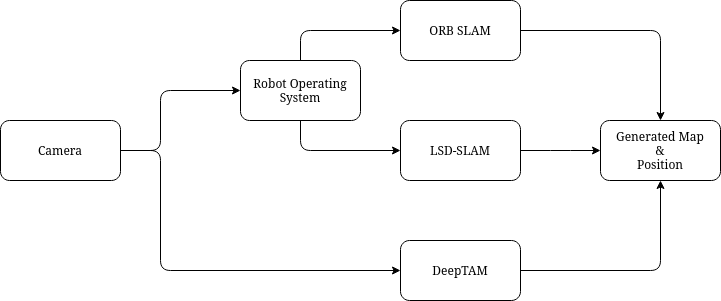
\includegraphics[width=1.0\linewidth]{media/images/illustrative_graph.png}
\end{center}
} \\

\textbf{\mbox{Accessibility of} \mbox{diploma thesis}} & 
{HTL Braunau archive, or\newline \url{https://diplomarbeiten.berufsbildendeschulen.at/}} \\



\end{tabularx}




%--------------------------------------------------------------------------------
% Unterschriften
%--------------------------------------------------------------------------------



\vspace*{\fill}

\textbf{Approval (date / signature)}

\fbox{
\begin{minipage}[t][3cm]{0.5\linewidth}
\centering
    Examiner \\
    %\hspace*{\fill}\includegraphics[width=0.8\linewidth]{fig/Unterschrift}\hspace*{\fill}
    \vfill
    \end{minipage}}
    \fbox{
    \begin{minipage}[t][3cm]{0.5\linewidth}
    \centering
    Head of College / Department
    \vfill
\end{minipage}
}

\restoregeometry



%	--------------------------------------------------------
% 	Eidesstattliche Erklärung
%	--------------------------------------------------------			
% !TEX root = ../Vorlage_DA.tex

%	########################################################
% 					Eidesstattliche Erklärung
%	########################################################


%	--------------------------------------------------------
% 	Überschrift, Inhaltsverzeichnis
%	--------------------------------------------------------
\chapter*{Statement}
%\addcontentsline{toc}{chapter}{Erklärung}


%	--------------------------------------------------------
% 	Inhalt
%	--------------------------------------------------------

I declare in lieu of oath that I have written this diploma thesis independently and without outside help, have not used sources and aids other than those stated directly and have made the sources used verbatim and in terms of content taken as such recognizable.
\vspace{3cm}

\begin{tabularx}{\textwidth}{l p{1cm} l p{1cm} X}


Braunau/Inn, \todayshort & & Alexander Voglsperger & & \hrulefill \\
\emph{Location, Date} & & \emph{Author} & & \emph{Signature} \vspace{2cm}\\ 

Braunau/Inn, \todayshort & & Simon Moharitsch & & \hrulefill \\
\emph{Location, Date} & & \emph{Author} & & \emph{Signature} \vspace{2cm}\\ 

\end{tabularx}




%	--------------------------------------------------------
% 	Inhaltsverzeichnis
%	--------------------------------------------------------			
\tableofcontents

%	--------------------------------------------------------
% 	Vorwort
%	--------------------------------------------------------	
% !TEX root = ../Vorlage_DA.tex
%	########################################################
% 							Vorwort
%	########################################################


%	--------------------------------------------------------
% 	Überschrift, Inhaltsverzeichnis
%	--------------------------------------------------------
\chapter*{Abstract}
% ENGLISH
An autonomous driving car has to orientate in the immediate vicinity. For this purpose the car needs a map and the own position in the map. Why is this such an important task when we already have technology like Global Positioning System (\gls{gps})? \gls{gps} provides routing data, but no live details what happens on the street, like an ongoing construction or a pedestrian crossing the street. To get this information the car has to collect visual data from its environment in real-time. This thesis examines two approaches of visual data processing to generate a map and locate the car inside this map. One approach is Simultaneous Localization And Mapping  (\gls{slam}), the other one uses artificial intelligence. The platform for ORB-\gls{slam} and LSD-\gls{slam} is the Robot Operating System (\gls{ros}), which handles the publish/subscriber based communication between the camera and the \gls{slam} algorithms.\newline
DeepTAM uses Deep Neural Networks which can learn to predict the distance between objects in an image. The prediction is based on training data. The accuracy of the result depends on the amount of training data. It is a system for keyframe-based dense camera tracking and depth map estimation that is entirely learned. This thesis shows how to implement the different algorithms in \gls{ros} and points out the pros and cons of each method compared to the others and gives an outlook into future methods.
\newline
\newline
\newline
\newline
% GERMAN
Ein selbstfahrendes Auto muss sich in der unmittelbaren Umgebung orientieren. Dazu benötigt das Auto eine Karte der Umgebung und die eigene Position. Warum ist dies so eine wichtige Aufgabe, wenn wir bereits über Technologien wie das Global Positioning System (\gls{gps}) verfügen? GPS liefert zwar die Standortdaten, aber keine aktuellen Details darüber, was auf der Straße passiert, wie z.B. eine Baustelle oder ein Fußgänger der die Straße überquert. Um diese Informationen zu erhalten, muss das Auto visuelle Daten aus seiner Umgebung in Echtzeit sammeln. In dieser Arbeit werden zwei Ansätze der visuellen Datenverarbeitung untersucht, um eine Karte zu erstellen und das Auto in dieser Karte zu lokalisieren. Ein Ansatz ist Simultaneous Localization And Mapping (\gls{slam}), der Andere verwendet eine künstliche Intelligenz. Die Plattform für den ORB-SLAM und den LSD-SLAM ist das Robot Operating System (ROS), das die Publisher/Subscriber-basierte Kommunikation zwischen der Kamera und den SLAM-Algorithmen übernimmt. Der DeepTAM verwendet ein Deep Neural Network, welches trainiert wurde den Abstand zwischen Objekten in einem Bild vorherzusagen. Die Genauigkeit der Vorhersage beruht auf der Anzahl der Trainingsdaten. Der DeepTAM verwendet ein angelerntes System welches mit Keyframe-basiertem Dense Camera Tracking und Tiefenschätzung eine Karte generiert. Diese Arbeit zeigt die Funktionsweise der verschiedenen Algorithmen, beleuchtet deren Vor- und Nachteile und gibt einen Ausblick auf zukünftige Methoden.

 

\addcontentsline{toc}{chapter}{Abstract}

%	--------------------------------------------------------
% 	Zusammenfassung
%	--------------------------------------------------------		
% !TEX root = ../Vorlage_DA.tex
%	########################################################
% 							Zusammenfassung
%	########################################################


%	--------------------------------------------------------
% 	Überschrift, Inhaltsverzeichnis
%	--------------------------------------------------------
\chapter*{Summary}
\addcontentsline{toc}{chapter}{Summary}

%	--------------------------------------------------------
% 	Inhalt
%	--------------------------------------------------------
This paper starts with the introduction into Simultaneous Localization and Mapping(SLAM) in general and two specific methods: ORB-SLAM and LSD-SLAM in detail. \newline
Next is the software which handles the communication between the individual algorithms called Robot Operatign System (\gls{ros}). It is a publish/subscriber based System. It contains tools like RQt and Rviz which are for visualizing the data. Afterwards there will be a detailed view into the structure and use of Artificial Neural Networks. Beginning with the components and then the most important types of Artificial Neural Networks for this task. Feed Forward Neural Networks and Convolution Neural Networks. The next step is Deep Learning. There are three different ways it can be implemented. Supervised, Semi-Supervised and Unsupervised. All of this methods need camera data. Therefore the Basler camera is explained . \newline
After the basics a more detailed look into the ORB-SLAM is taken to make it easier to understand the concept of the subsequent topic. The topics of the ORB-SLAM and LSD-SLAM include how the algorithm works, what data they require and in which way they can be used. Another art in this section is the DeepTAM and how it is structured and how it works. \newline
Last Section is the Workflow where the used hardware and software is listed, how it was setup, how the errors where handled that occurred during the project and how everything was used.

\pagebreak
\pagenumbering{arabic}	% Beginn mit arabischen Seitenzahlen

%	########################################################
%
% 						Arbeit	
%
%   Diesen Abschnitt an die eigenen Erfodernisse anpassen.		
%
%
%	########################################################

%	--------------------------------------------------------
% 	INFO: General Information for SLAMS
%	-------------------------------------------------------		
% Discription of what is a SLAM and what does it

\chapter{SLAM\authorA}

\section{What is SLAM?}
\gls{slam} is an acronym and stands for \textbf{S}iultaneous \textbf{L}ocalisation \textbf{A}nd \textbf{M}apping.
\emph{\enquote{\gls{slam} is concerned with the problem of building a map of an unknown environment by a mobile robot while at the same time navigating the environment using the map.}} \cite{slamfordummies} \newline
This problem is thus a chicken-and-egg problem because neither the map or location are known, and have to be estimated at the same time. Cameras, ultrasonic sensors and laser radar (\gls{lidar}) sensors are most commonly used for fetching the 2D and 3D data of the robot's surroundings \cite{arreverie}. \newline
There are several algorithms out there, which try to solve this problem using algorithms and some even deep learning. Mostly they achieve an approximate map, which is done in a reasonable time span. Many popular SLAM-algorithms use methods that include \textit{particle filters}, \textit{extended Kalman filter} and \textit{Covariance intersection}\cite{slamfordummies} \cite{1678144}. \newline

% Application environments of SLAMs
\section{Application}
The biggest selling point for using \gls{slam} implementations is pretty simple. Many places where autonomous robots may be required don't have good enough maps that are up-to-date , if the exist at all or it might be in an environment where positioning for instance GPS can't be used properly \cite{techapeekslam}. If slams weren't be used then someone would have to go to the place and make a map. This would delay the mission and add to the costs. \newline
With a robot, that is capable of using a SLAM method to detect and locate itself in the unknown surroundings this wouldn't be an issue. The robot could go in, generate a map that updates itself and use it to navigate around. \newline
Existing approaches that are used are in self-driving cars, unmanned aerial vehicles, autonomous underwater vehicles, planetary rovers and newer domestic robots.

% History of slams
\section{History}
The decisive work in \gls{slam}s was tone in the research by R.C. Smith and P. Cheeseman who worked on the representation and estimation of spatial uncertainty in 1986. Another major work in this area was done by a research group with the head being \textit{Hough F. Durrant-Whyte}. Durrant-Wyhte and his group showed that answer to \gls{slam}s lies in the nearly infinite amount of data that can be used. This lead to the motivation of finding algorithms which are trackable and approximate in a time realistic manner.\newline
Sebastian Thrun was playing.

% List and short information about  existing SLAMs
\section{Existing Methods}
There exits a big variety of \gls{slam} methods, that try to achieve the same goal using different approaches \cite{openslam}.
Most known or popular are the following:
\begin{itemize}
    \item \underline{EKF SLAM} \newline
    Utilizes the extended Kalman filter. The algorithm  uses the likely-hood for data association.
    It was the go-to \gls{slam} from 1990 to the early 2000s until Fast SLAM was introduced \cite{Fastslam}. 
    
    \item \underline{Fast SLAM} \newline
    Works recursively  so it scales logarithmically to the scale of the landmark. It can handle much bigger landmarks than the EKF-SLAM ever could without requiring as much computing power \cite{Fastslam}. 
    
    \item \underline{ORB-SLAM2} \newline
    It's a real-time \gls{slam} library for Monocular, Stereo and RGB-D cameras. It can detect loops and relocate the camera in real-time. It uses camera trajectory and sparse 3D reconstruction to get information out of the image sequence \cite{orbslam}.
    
    \item \underline{DVO-SLAM} \newline
    Implements a \textit{dense visual SLAM} system for RGB-D cameras. It's based on \textit{Dense Visual Odometry} and was extended to include frame-to-key matching with loop closure to older key-frames \cite{dvoslam1}. 
    
    \item \underline{RGB-D SLAM} \newline
    Utilizes the depth information of a \gls{rgbd-camera}, e.g., Microsoft Kinect or Intel Real-Sense Cameras \cite{rosrgbdslam}.
    
    \item \underline{LSD-SLAM} \newline
    It's a direct monocular \gls{slam}. It tracks the \textit{direct image alignment} and estimates geometry in form of \textit{semi-dense depth map} instead of relying on keypoints \cite{lsdslam_eccv}.
\end{itemize}

%	--------------------------------------------------------
% 	INFO: General information about the Robot Operating System
%	-------------------------------------------------------	
% Discription of what ROS is and what it does

\chapter{Robot Operating System\authorA}

\section{What is the Robot Operating System?}
The Robot Operating System, which is also known as \gls{ros} is a flexible framework for writing software that gets utilized on robots. It was founded by Willow Garage in 2012 and gets primarily maintained by the Open Source Robot Foundation (\gls{osrf}) \cite{osrf}. In Europe the project gets coordinated by the Fraunhofer IPA in form of the \textit{\gls{ros} Industrial Consortium Europe}. \gls{ros} is a middle-ware which is not a operating system but provides services that manage hardware abstraction, low-level device control, message-passing between processes and package management. \emph{\enquote{It is a collection of tools, libraries, and conventions that aim to simplify the task of creating complex and robust robot behavior across a wide variety of robotic platforms.}} \cite{aboutros}

\section{Design}
The processes of \gls{ros} are represented in nodes which are in a graph structure. Everything gets managed by a single process called \textit{\gls{ros} Master}, to whom all other nodes register on startup. But instead of sending all of the messages over the master, the master sets up a peer-to-peer connection between the nodes. This decentralized architecture is helpful as many robots consists of many computer hardware which is connected via a network and are likely to transfer big messages \cite{rosoneoone}. \newline
\begin{figure}[h]
	\centering
	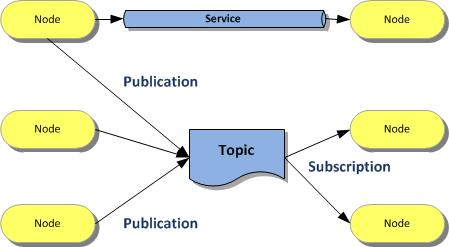
\includegraphics[width=0.7\textwidth]{./media/images/ros_structure.jpg}
  	\caption{\gls{ros} structure
  	\\Source: \url{https://tinyurl.com/tkf2smq}}
  	\label{rosstructure}
\end{figure}

\subsection{Topics}
It is based on a topic system, where a topic acts like a bus over which nodes send and receive messages. Each topic must be unique in it's name, which is usually set by the developer. The process of publishing and subscribing is handles anonymously so that no node knows which nodes are sending and receiving messages on a certain topic.

\subsection{Nodes}
A node, which represent a single running process, can provide data using a matching topic and publish it to the system, where theoretically every other node can subscribe to it, to get the data. 

\section{Licenses and OS}
The language-independent tools and the main client libraries have men released under the BSD license and as such they are open source software for commercial and research use. The majority of 3rd party packages are released under several other open-source licenses.\newline
The \gls{ros} libraries are geared toward a UNIX-System which is mainly due to their dependence on a large collection of open source software and libraries.
For example \textit{Ubuntu} is in the list of supported operating systems, while others like \textit{Fedora, MacOS and Windows} are \enquote{experimental} and are mainly supported by the community \cite{isrosforme}.

\section{Tools}
One of the core functionalities that \gls{ros} provides are the tools which allow the developers to visualize 2D and 3D data, record data, easily navigating \gls{ros} packages, creating complex scripts that configure and setup processes. Thanks to this tools it simplifies and provides solution for common robotic development.

\subsection{Rosbag}
Rosbag is a tool that can be used over the command line to record, playback and store \gls{ros} message data. The data gets stored in a file called bag, where it records the messages as they come in. It's possible to play these bag files. By doing this the recorded messages get published into the system, as they where live. It's very handy if you need data for later development or to use a bunch of different scenarios for testing

\subsection{RQt}
RQt provides a graphical overview of the \gls{ros} computation graph. It shows the nodes and how they are connected to each other. It also shows if a node is even subscribing to a topic or publishes something. Other than that it can be used to subscribe to different topics and show them directly in RQt.
\begin{figure}[h]
	\centering
	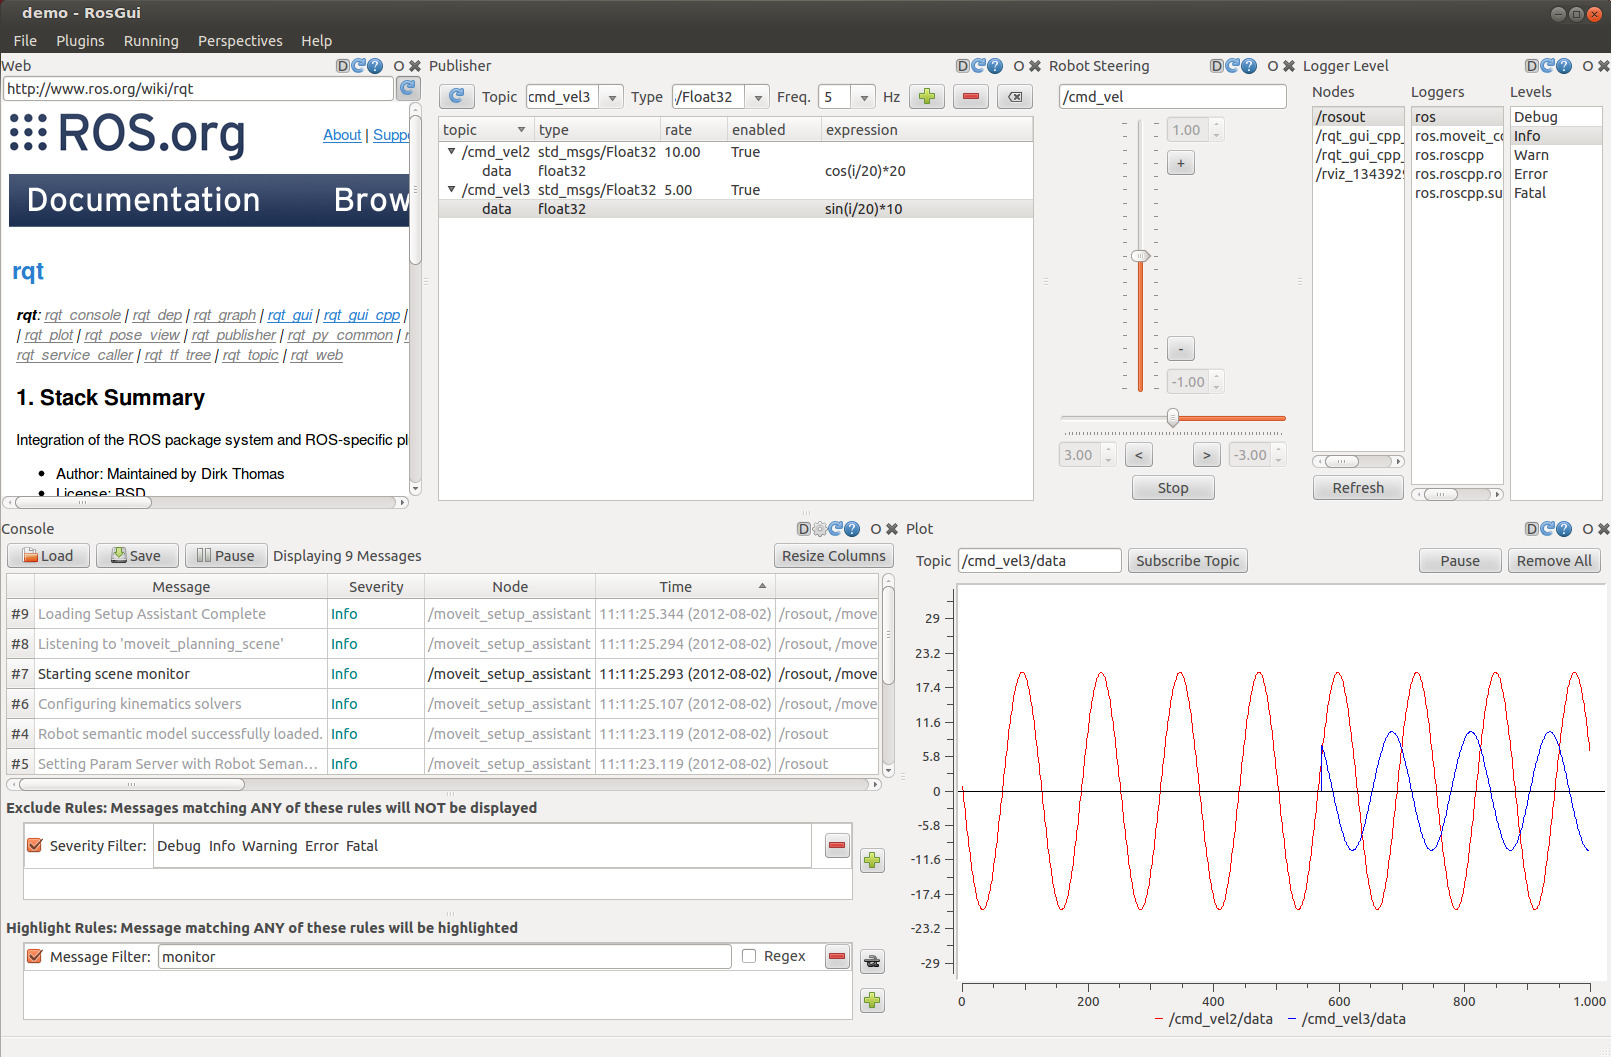
\includegraphics[width=0.6\textwidth]{./media/images/RQt}
  	\caption{RQt interface\\Source: \url{https://wiki.ros.org/RQt}}
  	\label{rqtinterface}
\end{figure}

\subsection{CatKin}
Catkin is the newer \gls{ros} build system, which compiles the files in the source folder. It is based on CMake and is cross-platform and language-independent as most other \gls{ros} tools.

\subsection{Rviz}
A visualizer for three-dimensional data where robots, environments and sensor information can be visualized. It is highly customise able with display many types of visualisation and plugin support. \newline
\begin{figure}[h]
	\centering
	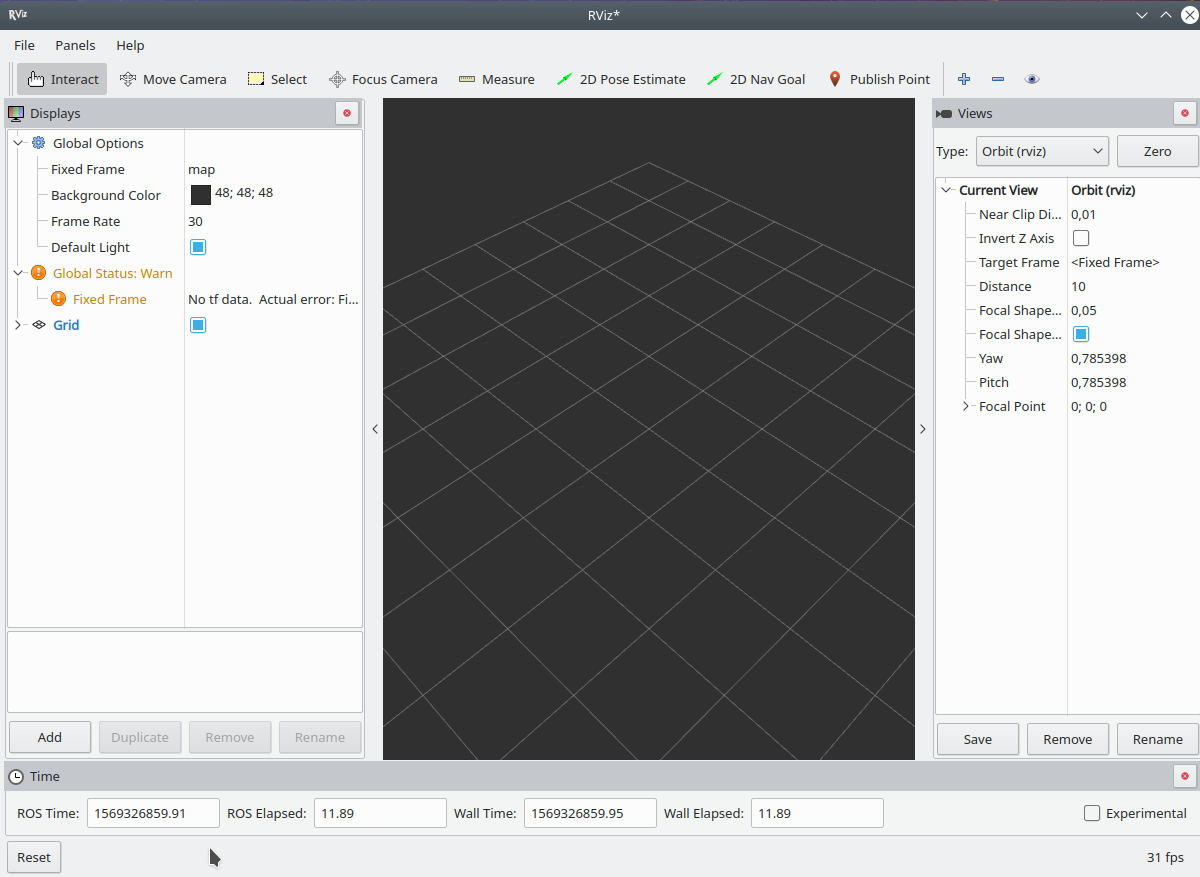
\includegraphics[width=0.7\textwidth]{./media/images/rviz}
  	\caption{Rviz interface}
  	\label{rvizinterface}
\end{figure}

\subsection{Roslaunch}
Roslaunch is a tool for launching multiple \gls{ros} nodes and setting parameters on startup. It can be used to launch nodes locally or remotely on a server.
The configuration for a start script is written in a launch file using XML. In these files it's easy to make a automated startup and configuration process to be executed with one command. It's possible to execute launch files in other launch files to chain them together.

%	--------------------------------------------------------
% 	INFO: General information about artificial neural networks
%	-------------------------------------------------------		
% Discription of what is a Artificial Neural Networks and what does it
\chapter{Artificial Neural Networks\authorB}

\section{What is a Artificial Neural Networks?}

  \textbf{A}rtificial \textbf{N}eural \textbf{N}etworks(ANN) are inspired by biological neural networks that constitute animal brains. Important to notice is that they are not faithful models of biologic neural or cognitive phenomena. In fact most of these models are more closely related to mathematical and/or statistical models(For Example: clustering algorithms). Such systems "learn" to perform tasks by considering examples, generally without being programmed with task-specific rules. 
 
\section{Areas of Application}

 ANN are viable computational models for a wide variety of problems, including pattern classification, speech synthesis and recognition, adaptive interfaces between human and complex physical system, function approximation, associative memory, clustering, forecasting and prediction, combinatorial optimization, nonlinear system modeling, and control
 \cite{fundamentals_ann}
 
\section{Components of an ANN}

Simplified a ANN consists of these components: neurons, connection and the weight associated with them, the propagation function, a loss function and a bias. The following topics will give you a short summary what these components are and afterward is an explanation  how they work together. 

\subsection{Neurons}

Neurons are elementary units in an ANN. A neuron gets one ore more inputs and depending on the value of the inputs the output is set. A neuron can get its inputs from other neurons or, if its at the beginning, from the source of the data that needs to be processed. Depending on the Type of ANN they are placed in different structures. In most cases the output of a Neuron is a number between 0 and 1.

\begin{figure}[h]
	\centering
	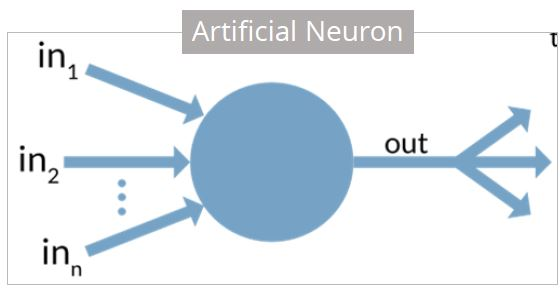
\includegraphics[width=0.7\textwidth]{./media/images/diagram-for-general-view-of-artificial-neuron.jpg}
  	\caption{General view of Neurons
  	\\Source: https://tinyurl.com/yyfthk7c}
  	\label{Gvon}
\end{figure}

\subsection{Connection and weights}

These Neurons are Connected. Which neurons are connected with others depends on the structure. The weights characterize how important a connection between neurons is. 

\textbf{For example:}\newline
A neuron, we call it base for this example, has two neurons connected to it as inputs. The weight of the connection of the first neuron has a bigger weight than the second connection. That means the output of the base depends more on the input of the first neuron 

\subsection{Propagation function  and activation function}

This is a function witch takes the Inputs of a neuron, the weight of these connections and the bias and adds them up. The resulting value is the processed by the activation function which sets the output. One of the most common activation function is the sigmoid function because it is not a step function which means the output does not  change instantaneously. That is important for the training algorithm.

\subsection{Bias}

The bias is a Neuron which has no Inputs. A bias is used to shift the decision boundary to the left or right.

\section{Organization}

A artificial neural network can be organized in many different ways.

\subsection{Feed Forward ANN}

\begin{figure}[h]
	\centering
	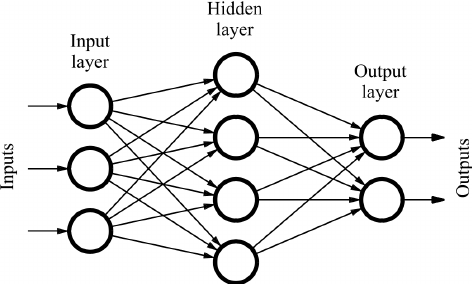
\includegraphics[width=0.7\textwidth]{./media/images/feed_forward_neural_network.png}
  	\caption{Feed forward network}
  	\label{ffNN}
\end{figure}

The following picture demonstrates a feed forward ANN .There are a variable number of hidden layers depending on the purpose of the neural network. Nothing in the hidden layer is visible. 

\subsection{CNN}

Convolution Neural Network (CNN) is the most important Network organization for this task. It is based on the human visual cortex and perfect for image and video recognition. The components of a CNN are a series of convolution and sub-sampling layers followed by a fully connected layer and a normalizing layer.

How a CNN works will be explained in the following example. The same example like in "Review of Deep Learning Algorithms and Architectures"\cite{networks,exampleCNN} will be used
\begin{figure}[h]
	\centering
	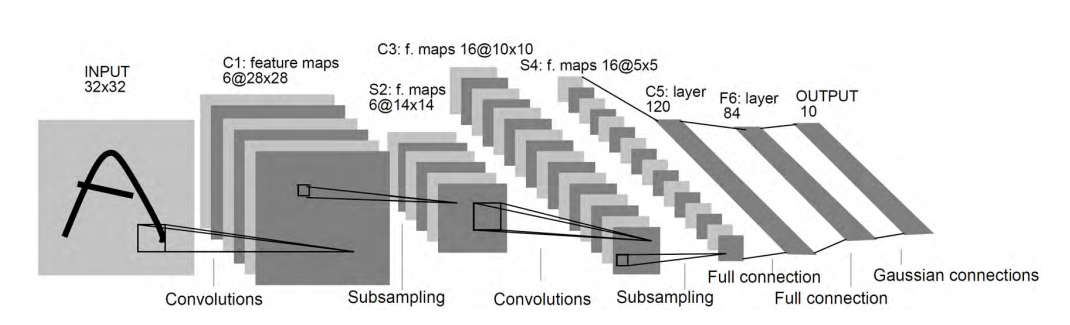
\includegraphics[width=1.1\textwidth]{./media/images/CNN.PNG}
  	\caption{7-layer architecture of CNN for character recognition
  	\\ \cite[Fig.~4.]{networks,exampleCNN}}
  	\label{CNN}
\end{figure}

Progressively more refined feature extraction at every layer is performed by the series of multiple convolution layers. This process is moving from input to output layer. After the convolution layers there are fully connected layers that perform classification. There is also the possibility of putting Sub-sampling or pooling layers between each convolution layer. The input of a CNN is a 2D n*n pixelated image. Each layer consists of filters or kernels (groups of 2D neurons). In most neural networks neurons in each feature extraction layer are connected to all neurons in the adjacent layers. But in a CNN they are only connected to the spatially mapped fixed sized and partially overlapping neurons in the previous layer’s input image or feature map.

\section{Encoder-Decoder-Based Architecture}

Encoder-Decoder-Based networks are networks, which try to reconstruct their own input. You construct the network so that it reduces the input size by using one or more hidden layers, until it reaches a reasonably small hidden layer in the middle. As a result your data has been compressed (encoded) into a few variables. From this hidden representation the network tries to reconstruct (decode) the input again.

In order to do a good job at reconstructing the input the network has to learn a good representation of the data in the middle hidden layer. This can be useful for dimensionality reduction, or for generating new “synthetic” data from a given hidden representation. This is especially important considering that we are trying to construct a 3D Map out of the Camera Input. 












%	--------------------------------------------------------
% 	ORB-SLAM
%	--------------------------------------------------------		
% Discription of what ORB-SLAM is, how it works and implementation

\chapter{ORB-SLAM2\authorA}

\section{What is ORB-SLAM?}
ORB-SLAM2 is a versatile, real-time SLAM implementation which uses Mono-, Stereo- and RGB-D cameras. It's designed to generate a 3D map from prominent points in the picture and keypoints. It features loop closing, re-localization and a reusable map.\cite{orbslam2} It works in a wide variety of use cases. The SLAM can be used on a small hand-held camera or drones up to self driving cars.
ORB-SLAM2 is based on ORB-SLAM and was inter alia developed by Raúl Mur-Artal who already worked on ORB-SLAM.

\section{How does the ORB-SLAM work?}

\subsection{Extracting Keypoints}
The SLAM uses a feature-based method. This means that it extracts features on prominent keypoints throughout the image input. These feature information is then distributed to all operations which handle them independent from the camera type. \cite{orbslam2} \newline\newline


This is how finding these keypoints works on different camera types:
\begin{itemize}
    \item \underline{Stereo Image} \newline
    For a stereo camera setup the keypoints get extracted for both images separately and then the left keypoints are searched on the right image. Then the found points get compared to the original ones that where found on the right side
    \item \underline{RGB-D Image} \newline
    On a RGB-D camera keypoints get extracted using prominent keypoints and then calculating the approximate position using the depth information from the information from the depth sensor.
    \item \underline{Monocular Image} \newline
    On a Monocular image the approximate position gets triangulated by using multiple images. The Disadvantage is that they don't provide a scale information and only do rotational and transnational movement estimations.
\end{itemize}

\subsection{Loop-closing and Bundle Adjustments}
Loop-closing and bundle adjustments are performed in two steps. First the loop-closing will happen when the system detects overlapping environments where the system changes scaling to reconnect certain parts as scale drifting will occur on monocular cameras.\newline
Second step is the bundle adjustment, which gets executed after a successful loop-closing, where the system tries to optimize all keypoints and keyframes using the Levenberg-Marquardt method (alternative to Gauss-Newton method).\cite{LevenbergMarquardMethod} Also the camera orientation and position will be optimized to compensate errors in tracking. All the bundle adjustment is done in a separate thread since this is a heavier task.\newline
When finished, the updated and optimized keyframes and keypoints get merged into the original keyframes and keypoints.\cite{orbslam2}

\subsection {Localization}
When a area has been mapped well in the past the \textit{Localization Mode} can be turned on which deactivates the Local Mapping and the Loop Closing thread and this saving computing power.
Locating is done by continuously comparing the previous points with the current points of the image. This works when an area is unmapped but drifting might add up.
Matching the current points with the one on the map will ensure that it is drift-free.\cite{orbslam2}

\subsection{Input/Output}
\textbf{Input Data:} rectified Monochrome/Color images\newline
\textbf{Output Data:} Rough 3D map with keypoints and keyframes and image with current prominent points

%	--------------------------------------------------------
% 	LSD-SLAM
%	--------------------------------------------------------		
% Discription of what LSD-SLAM is, how it works and implementation

\chapter{LSD-SLAM\authorA}\label{ref:lsdslam}

\section{What is LSD-SLAM?}
LSD-SLAM stands for \textbf{L}arge-\textbf{S}cale \textbf{D}irect Monocular \gls{slam} and is a fairly new real-time monocular \gls{slam} that is fully direct-driven instead of relying on keypoint/keyfeature \cite{lsdslam_eccv}. The algorithm works on the image intensity for tracking and mapping at the same time.\newline
This method allows building large-scale maps on normal processors that are consistent when comparing it to current state-of-the-art algorithms. \newline

\begin{figure}[h]
	\centering
	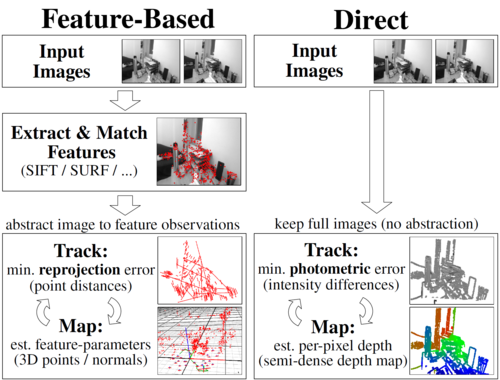
\includegraphics[height=0.5\textwidth]{./media/images/direct-vs-feature-based.png}
  	\caption{Feature-Based and Direct Difference
  	\\Source: \url{https://tinyurl.com/ycmjhb9d}}
  	\label{featurebased_direct_difference}
\end{figure}

\section{Difference Feature-Based and Direct}
\begin{itemize}
    \item \underline{Feature-based} \newline
        A feature-based \gls{slam} (e.g. ORB-SLAM \ref{ref:orbslam}) looks for distinctive points in the image and then uses only these keypoints to process the information. When there are only a few prominent keypoints (e.g indoor, tunnels) the result will not be that accurate.
    \item \underline{Direct} \newline
        Direct based \gls{slam}s use all information that's provided in the image. This does not only include distinctive points but also edges and sometimes surfaces and thus makes it possible to create a more accurate and denser 3D map \cite{lsdslam_eccv}.
\end{itemize}
\begin{figure}[h]
	\centering
	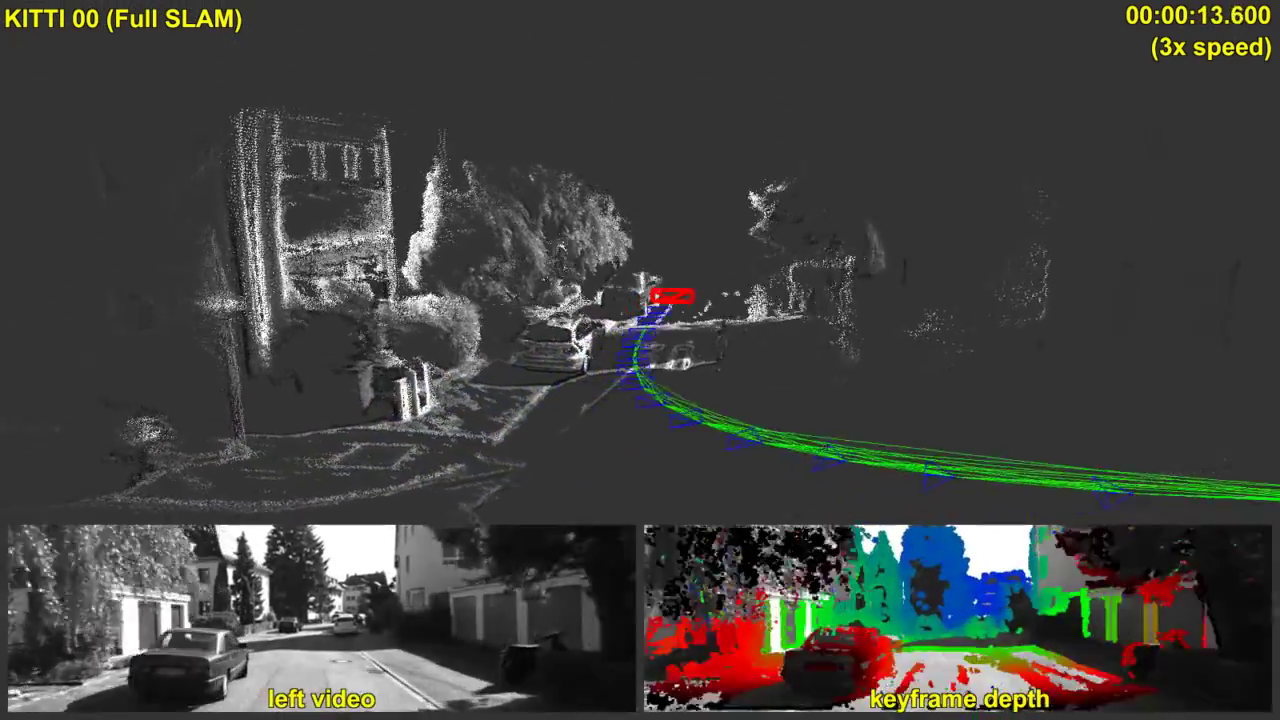
\includegraphics[width=0.7\textwidth]{./media/images/lsd-slam.png}
  	\caption{LSD-SLAM Example image
  	\\Source: \url{https://tinyurl.com/qkuamyy}}
  	\label{lsdslam}
\end{figure}

\section{How does the LSD-SLAM work?}
\subsection{Components that make up the LSD-SLAM}
\begin{itemize}
    \item \underline{Tracker} \newline
        The \textit{Tracking} component uses the current frame in relation to the last frame to continuously track the camera movement.
    \item \underline{Depth Map Estimation} \newline
        \textit{Depth map estimation} is done using tracked frames to refine or replace the current frame. Depth information is calculated by filtering over a small per-pixel baseline. If the camera has moved too far or the image has changed too much a new keyframe is initialized \cite{lsdslam_eccv}.
    \item \underline{Map Optimization} \newline
        When a keyframe gets replaced as a tracking reference, the refinement process stops and it gets included in the 3D depth map. \textit{Map optimization} then starts working to detect loop-closures or scale-drifts. This is done by a similarity transformation to frames that where taken nearby.
\end{itemize}

\subsection{Depth Map Estimation}
New keyframes are created when there where no frames before or the camera has moved/rotated so far that the set threshold has been exceeded. When this happens the new latest frame is chosen to become the new keyframe and the keypoints from the previous keyframe get projected onto the new one. The process is followed by scaling to fit the needs of the Direct Image Alignment. When that is done the keyframe replaces the previous ones and gets used to track the subsequent frames.\newline
Not every frame results in a new keyframe. Frames that don't make it to a new keyframe are used to improve and refine the current keyframe. The refinement is done by using a small stereo comparison for regions in an image where the expected use for advancement is higher. The result of this comparison then gets merged into the existing 3D point cloud to add potentially new information or refining existing pixels \cite{lsdslam_eccv}.

\subsection{Map optimization}
Scaling, rotation and movement isn't always perfect, which results in drift. Even if the drift effect is little it adds up, which might result in some very off map \cite{lsdslam_eccv}. The Pose-Graph-Optimization is a optimization algorithm which aims to fix these drifts with pretty good results. The advantages of the pose-graph-optimization are that it's fast and vulnerable for poor initialization estimates \cite{posegraphoptimization}. \newline

\begin{figure}[h]
	\centering
	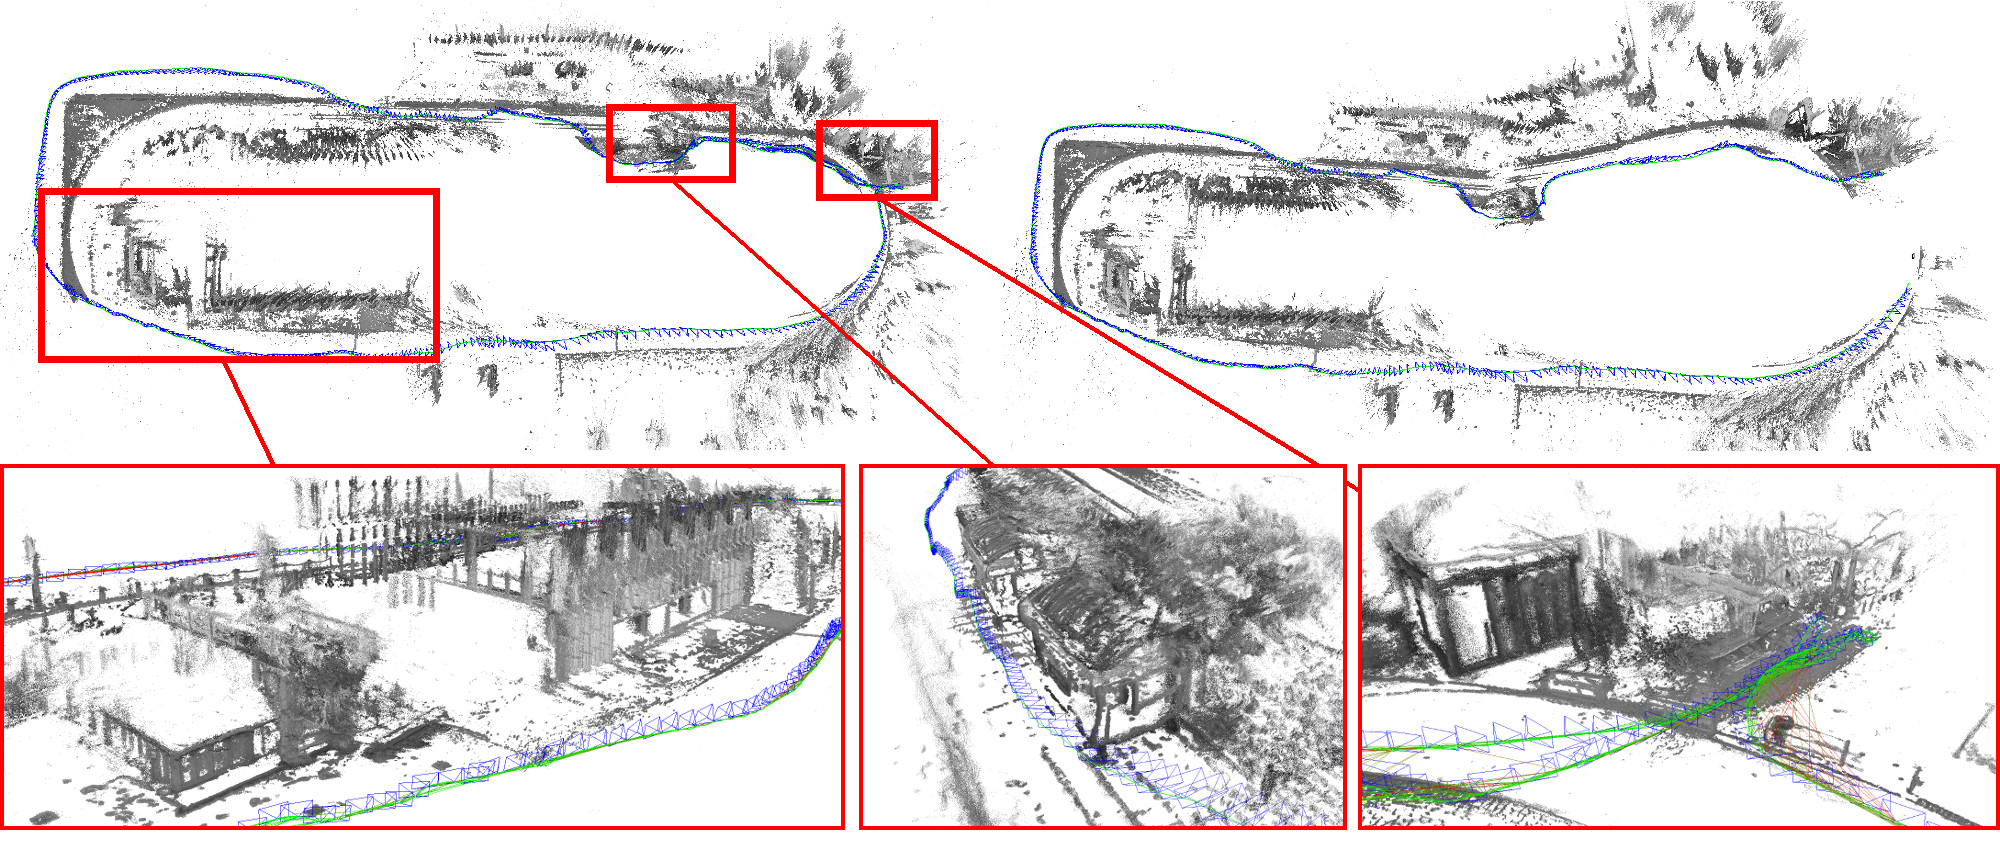
\includegraphics[width=0.8\textwidth]{./media/images/lsd-slam-pose-graph-optimization.jpg}
  	\caption{LSD-SLAM Pose-Graph-Optimization (left after loop-closure, right before loop-closure)
  	\\Source: \url{https://tinyurl.com/qkuamyy}}
  	\label{lsd-pose-graph-optimization}
\end{figure}

\subsection{Input/Output}
\textbf{Input Data:} rectified monocular image, camera info\\
\textbf{Output Data:} image with probability colored points, 3D point cloud

%	--------------------------------------------------------
% 	Deep TAM
%	--------------------------------------------------------		
\chapter{DeepTAM\authorB}

\section{What is DeepTAM?}
DeepTAM provides a keyframe-based dense camera tracking and depth map estimation system that is entirely learned. The idea of DeepTAM is based on DTAM \cite{dtam}.The generic idea is: drift-free camera tracking via a dense depth map towards a keyframe and aggregation of depth over time. But the way to implement this concept is different. In the DeepTAM deep networks are used for tracking and mapping.These networks learn only from data. It also processes more than two images for the 6 DOF egomotion and depth estimation. With that it can avoid the drift of the use of keyframes and as more keyframes come in it can refine the depth map.

\section{Tracking}

The main objective is to estimate a 4 x 4 transformation matrix T. This matrix maps a point in the keyframe coordinate system to the coordinate system of the current camera frame.
\newline
DeepTAM uses an more efficient way. It generates a virtual keyframe and tries to predict the increment instead of trying to estimate T. For more details see \cite{ZUB19a}.

\subsection{Network Architecture}
To estimate the 6 DOF pose between a keyframe and an image the encoder-decoder-based architecture is used. To estimate camera motion you have to relate the keyframe to the current image. Because of that DeepTAM uses optical flow as an supportive task. With this optical flow the network is ensured to take advantage of the relationship between both frames. It uses two network branches for predicting the pose. One is the optical flow prediction and the other is the pose hypotheses generation. This improves the accuracy for the pose prediction.

\section{Mapping}
\gls{optical-flow}





%	--------------------------------------------------------
% 	Workflow
%	-------------------------------------------------------	
\chapter{Workflow}


% ---------------------------------------------------
% USED HARDWARE
\section{Used Hardware\authorA}
For video capturing a \textit{Raspberry Pi 3B+} with a \textit{Pi Camera V2} or a \textit{Pi Wide Angle Lens Camera} are used. The Raspberry Pi sends the video feed to a separate more power full PC over WiFi using a Python3 script. \newline
For processing a \textit{Lenovo Think-Station S20} or a \textit{Lenovo W550s} are used depending on the amount of processing power is required. For more intense work a server access at the Johannes Kepler University was supplied to work on their system. \newline
As the work is based around implementing it on the Audi Autonomous Driving Cup (\gls{aadc}) car a remote controlled model car was borrowed for a few weeks.


% ---------------------------------------------------
% USED SOFTWARE
\section{Used Software\authorA}
\subsection{Raspberry Pi}
The Raspberry Pi is running Raspbian Buster since it is well optimized for the mini computer and only required to be able to execute a Python script to send the raw video feed over http to the the processing device.\newline
\subsection{PC}
The Think-Station and the laptop are running Kubuntu 18.04, which is basically Ubuntu but has a GUI that's a more like Windows and is supported until May 2023. \newline
The Think-Station has a eight core Intel Xeon CPU, a GTX 1660TI and 12GB of RAM inside. \newline
The Laptop has a four core Intel i7 and 8GB of RAM built in.\newline

\textbf{\underline{ADTF}} \newline
At first Ubuntu 16.04 with Automotive Data and Time-Triggered Framework (\gls{adtf}) was used since it's the recommended environment by the \gls{aadc} car manufacturer DigitalWerk. There were many compatibility ans stability issues and it is very difficult to get into the whole system as it's not very beginner friendly. After trying to get the basics of \gls{adtf} working it was clear that switching to ROS might be better. The main problems with \gls{adtf} are, that \gls{adtf} isn't running very stable, requires certain packages to be in a non-standard folders and not having them in the regular location and it is very difficult at the when using it for the first time.

\textbf{\underline{ROS}} \newline
Running ROS Melodic on Kubuntu 18.04 was pretty straight forward. The instructions on the ROS website are very clear and can be directly copied without issues. The principle of the workspace is also easy to understand. In the source folder the modules get put in and when compiling the modules automatically generates a setup file to use them. Usage is very easy as the framework already does a lot in the background and using nodes is nearly always setting input and output with a few parameters.


% ---------------------------------------------------
% Setup
\section{Setup\authorA}
As the PC and laptop are not the best idea to run around with, a Raspberry Pi is used instead to stream the video over WiFi to the PC/laptop which are connected to the router over LAN. This makes the camera setup very portable as the pi, camera and powerbank are packed together and don't have much weight. The PC can sit somewhere where and just processing the received video signal.
\begin{figure}[h]
	\centering
	\includegraphics[width=0.8\textwidth]{./media/images/PiSetup.png}
  	\caption{Stream setup with Raspberry Pi, camera and powerbank}
  	\label{picamssetup}
\end{figure}

% ---------------------------------------------------
% SENDING IMAGE FROM RASPBERRY PI TO PC/LAPTOP
\section{Streaming video from Pi to PC\authorA}

\subsection{Enabling Camera}
To use a camera on a Raspberry Pi the interface needs to be enabled first. This can be done in the built-in tool called \textit{raspi-config}. In this tool under the subsection called \textit{Interfacing Options} there is a option with the name \textit{Camera}. When this is done the camera can be used after a restart.

\subsection{Python Script}\label{ref:streamPythonScript}
In the code snipped \ref{code:videostreamMain} at first a \textit{piCamera} instance with the name \textit{cam} is created. As parameters the resolution gets set to \textit{1280x720} pixels and the frame rate is set to \textit{30} frames per second (\gls{fps}). If needed the image can be rotated, e.g the camera is mounted upside down. When starting the camera a output and format are expected. For the output a separate class is used which sets how and when a new frame can be published and for the format the \textit{mjpg} video codec is chosen, as a pack for getting MPEG-streams already exists in \gls{ros} and it's not power hungry when running it on the Raspberry Pi. \newline
After the camera \enquote{recording} has started successfully the server is started to make the stream accessible to other devices. The server runs until the user closes the script using \textit{CTRL + C}. After closing the server the \textit{finally} block gets called, where the camera \enquote{recording} is stopped so that other programs can use the camera again.\newline
\lstinputlisting[language=Python, firstline=77, lastline=91,caption={Main Function of Camera Feed},label={code:videostreamMain}]{./media/code_snippets/HTTPCamStream.py}

The streamingHandler that is shown in snipped \ref{code:videoStreamHandler} handles the actions that are taken when client connects to the Raspberry Pi. At the beginning it checks if the client is requesting the \textit{/stream.mjpg} file. If the client is not requesting that specific file a \textsc{404 Not Found} Error is returned. But if the correct file is requested at first a \textsc{200 OK} code. In addition to the status code headers are send, which tell the client to not use cache. After sending the \textsc{HTTP OK} to the client a permanent loop is started which always waits until a new image from the camera is ready and then sends it to the client as an JPEG image. The loop ensures that the always client receives the latest image and so creates a video. Should the client drop the connection an exception is raised which causes the loop to stop and end the handler for that specific client until the client connects again.\newline
\lstinputlisting[language=Python, firstline=42, lastline=74, caption={Streaming Handler of CamStream},label={code:videoStreamHandler}]{./media/code_snippets/HTTPCamStream.py}

The behavior when a new image from the pi camera is ready to send is defined in the snipped \ref{code:videoStreamingOutput}. At the beginning it initializes itself with basically no image. \textit{piCamera} class constantly writes into this, as it's defined as the output. When a new image is ready the \textit{picamera} class sends \enquote{\textbackslash xff\textbackslash xd8} as binary to the output class to notify it. The output class then cuts the buffer so it only contains the current image and sets it in the \textit{frame} variable. To let everybody else know that a new image is ready it sends out a notification.\newline
\lstinputlisting[language=Python, firstline=26, lastline=40, caption={Streaming Output of CamStream},label={code:videoStreamingOutput}]{./media/code_snippets/HTTPCamStream.py}


% ---------------------------------------------------
% RECEIVING IMAGE ON PC/LAPTOP
\section{Receiving images on PC and Laptop\authorA}
For receiving the images on the PC or Laptop an existing \gls{ros}-node is used. Video-Stream-OpenCV is designed to publish videos in the \gls{ros} network which are received from different sources, e.g. USB-cameras, video-files, network cameras and video-streams \cite{videostreamopencv}.

\subsection{MJPG-Stream receiver}
To automate the startup procedure of the node a roslaunch file is used to start the node is written for and automatically sets the required parameters.\newline
The launchfile shown in \ref{code:mjpgstreamreceiverlaunch} published the received image stream on a topic called \textit{camera}. The video stream provider are the Raspberry Pi's IP-address, port and \textit{/stream.mjpg} directory. 30 \gls{fps} are used since they provide a good balance between amount of traffic and amount of detail in the movement.\newline
\lstinputlisting[language=XML, firstline=3, lastline=14, caption={MJPG-Stream receiver Launch file},label={code:mjpgstreamreceiverlaunch}]{./media/code_snippets/mjpg-stream.launch}


% ---------------------------------------------------
% Cameras
\section{Cameras\authorA}
Nearly every camera has some kind of distortion where the proportions of the image are different to the real world. This is especially noticeable on wide angle lenses which can capture a bigger part of the environment while sitting in the same spot. This can be seen in figure \ref{cameracomparison} that the normal camera only captures a small portion compared to the wide angle lens camera but the wide angle lens creates distortions when getting to the edges.
\begin{figure}[h]
	\centering
	\includegraphics[width=0.8\textwidth]{./media/images/CameraComparison.png}
  	\caption{\textbf{Left Image:} normal Raspberry Pi Camera. \textbf{Right Image:} wide angle lens camera}
  	\label{cameracomparison}
\end{figure}

\subsection{Calibration}
To get rid of the distortions on a wide angle lens camera calibration is needed, which is a mask that gets applied on the image to remove these distortions and rectify it.
For calibration the \textit{camera calibration}-node is used.  Calibration is done by moving and rotating a checkerboard is used since it has good contrast between the tiles and the size of a tile is known and always the same. The node recognizes the checkerboard and calculates the distortion-factors from a series of pictures that have been taken.\newline
The command for starting the node is the following, where amount of tiles, size of tiles in millimeter and camera are set:\newline
\begin{lstlisting}[language=BASH,caption={Start Calibration Node}]
rosrun camera_calibration cameracalibrator.py --size 8x6 --square 0.026 --no-service-check image:=/camera/image_raw camera:=/camera
\end{lstlisting}

This command opens a window which shows the live image feed from the camera and highlights edges on the checkerboard which is shown in figure \ref{img:cameracalibration}. These highlighted edges are points which are used to calculate the distortion parameters using an algorithm that was developed by \href{https://docs.opencv.org/2.4/doc/tutorials/calib3d/camera_calibration/camera_calibration.html}{OpenCV} \cite{cameracalibrationopencv}.
\begin{figure}[h]
	\centering
	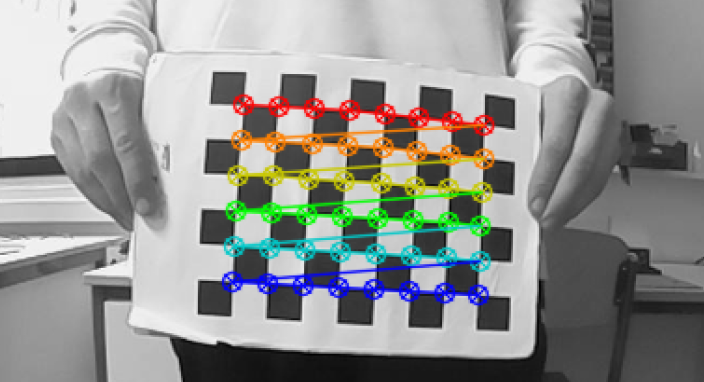
\includegraphics[width=0.8\textwidth]{./media/images/CameraCalibration.png}
  	\caption{Camera calibration}
  	\label{img:cameracalibration}
\end{figure} \newline

When the node has enough reference images the computing of the parameters can start. The duration of the calculations depends on the CPU and how many images have been taken. But most likely it will take around 5 Minutes until the computing is finished. The output data contains two formats of the same data which will look something like shown in figure \ref{code:calibrationyaml}. The output files are normally compatible with all applications without any issues.\newline
\lstinputlisting[language=XML, firstline=1, lastline=14, caption={Calibration file},label={code:calibrationyaml}]{./media/code_snippets/calibration.yaml}


% ---------------------------------------------------
% Running Monocular ORB-SLAM2
\section{Running Monocular ORB-SLAM2\authorA}\label{ref:runningmonocularorbslam}
Integrating ORB-SLAM2 \ref{ref:orbslam} is pretty straight forward since there is already \gls{ros} version of it which is very well maintained by \textbf{Lennart Haller} on behav of \textit{appliedAI-Initiative} on \href{https://github.com/appliedAI-Initiative/orb_slam_2_ros}{GitHub} \cite{orbslam2rosgithub}. It just needs to be cloned into the \textit{src} folder of the \gls{ros}-workspace and complied using the \textit{catkin build} command.When building the packs is finished the generated setup-file has to be sourced. The file is located under \textit{workspace/devel/setup.sh} and can be sources using the \textit{source setup.sh} command. After sourcing the setup all new types of commands that are added by the nodes are available.

\subsection{Calibration file}\label{ref:calibrationorbslam}
Before using the ORB-SLAM the calibration file needs to be created in \textit{src/orb\_slam2/config/config.yaml}. For a baseline the config from another mono-camera can be copied. The calibration part looks like shown in \ref{code:orbslamconfig} and thus the config that the calibration tool generated needs to be converted manually. In the camera\_matrix the values are the following:
\begin{lstlisting}[language=XML,caption={Matrix listing},label={code:calibrationmatrix}]
	  	[camera.fx, 0, camera.cx, 0, camera.fy, camera.cy, 0, 0, 1]
\end{lstlisting}
The distortion\_coefficients need to be mapped like shown in listing \ref{code:calibrationdistortionmatrix}.
\begin{lstlisting}[language=XML,caption={Matrix listing},label={code:calibrationdistortionmatrix}]
	  	[camera.k1, camera.k2, camera.p1, camera.p2, 0]
\end{lstlisting}
Additionally the width, height and \gls{fps} of the incoming video have to be set to use the correct amount of frames and resolution.\newline
\lstinputlisting[language=XML, firstline=3, lastline=17, caption={ORB-SLAM2 config calibration}, label={code:orbslamconfig}]{./media/code_snippets/config.yaml}

\subsection{Launching ORB-SLAM2}
To load the new config file a new launch file is the best way to tell the \gls{slam} to use this config instead of the default parameters. The launch files for ORB-SLAM2 sit in \textit{src/orb\_slam2/ros/launch} where an existing one can be duplicated. The new launch-file should look like the snipped \ref{code:orbslam2launch} except in line \textbf{13} the wrong config is specified. Additionally in the config other settings can be set. For example if the node should publish a pointcloud or position, only do tracking. It is also possible to load an existing map which has been created before and might be used to add additional information or do tracking only on it. When everything is configured it is now possible to launch the ORB-SLAM2 using \textit{roslaunch orb\_slam2\_ros orbslam.launch}. \newline
\lstinputlisting[language=XML,  caption={ORB-SLAM2 launch file}, label={code:orbslam2launch}]{./media/code_snippets/orbslam.launch}

When starting RQt \ref{rqt} and opening the \textsc{Node Graph} it should show, like seen in figure \ref{img:nodegraphstreamorbslam} that the camera-node is sending \textit{image\_raw} to the \textit{orb\_slam2\_mono}-node. If that is not the case it is most likely due to some spelling error or a \textit{remap} line in the launch-file of the ORB-SLAM2.\newline
\begin{figure}[h]
	\centering
	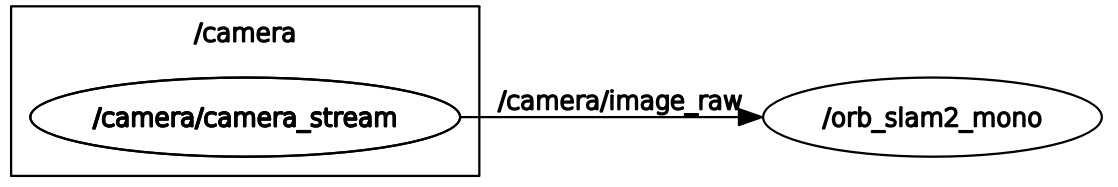
\includegraphics[width=0.8\textwidth]{./media/images/nodegraphstreamorbslam.png}
  	\caption{Node Graph with Stream and ORB-SLAM}
  	\label{img:nodegraphstreamorbslam}
\end{figure}


% ---------------------------------------------------
% Running Stereo ORB-SLAM2
\section{Running Stereo ORB-SLAM2\authorA}
As explained in the ORB-SLAM chapter \ref{ref:orbslam} there are some problems with running it with a single-camera setup. The main problem is that on a monocular image the scale information is not provided an thus drifting occurs. A way to bypass this problem is by using two cameras looking in the same direction but with a slight offset. This then is works a bit more like eyes where the depth perception is easier when having both eyes open compared to only having one open.

\subsection{Hardware setup}
Since stereo cameras and synchronization boards are not cheap, two identical Raspberry Pi's with the same camera are used for the testing environment. The two Raspberry Pi's have the same SD card type, operating system and packages to prevent any timing difference as much as possible. The Cameras are taped on a stick of wood with a distance of around six centimeters to mimic the average distance between the human eyes.

\subsection{Calibration}
Calibration in this testing environment is pretty straight forward as the cameras used are the normal Pi Cameras v2 which basically have little to no distortion. Just for being on the save side calibration was done on both cameras and the values only are slightly different. So the format that was entered in the config was the same as on the monocular \gls{slam} calibration \ref{ref:calibrationorbslam}. If cameras with distortion are used there are more values that are required a bit further down in the config.

\subsection{Software setup}
The same Python script as already explained in section \ref{ref:streamPythonScript} is used on both devices to make the camera feed available on the local network. To receive these streams two MJPG-Stream receivers are required. The thing to note here is that the camera name must be unique, e.g they may be named \textsc{lcamera} \ref{code:leftcameralaunch} and \textsc{rcamera} \ref{code:rightcameralaunch} to know which is the left and right camera. Also required is to set the stream receiver to the correct IP-address since it is important later. Re-building isn't necessary since only the config and launchfile change, which are not compiled but instead loaded every time the \gls{slam} starts.\newline
\begin{lstlisting}[language=XML,caption={Left camera stream launch file},label={code:leftcameralaunch}]
	  	<arg name="camera_name" value="lcamera" />
\end{lstlisting}
\begin{lstlisting}[language=XML,caption={Right camera stream launch file},label={code:rightcameralaunch}]
	  	<arg name="camera_name" value="rcamera" />
\end{lstlisting}

Since the two video streams are still on a topic that the \gls{slam} doesn't subscribe on it is necessary to remap the two streams to the correct topics. This can be done in a launchfile for the stereo ORB-SLAM.
To do this it is only required to add two lines which are shown in listing \ref{code:stereoorbremap} at line \textbf{5} and \textbf{6} before all other settings for the \gls{slam} get set. This remaps the nodes that triesw to subscribe to e.g \textit{/image\_right/image\_color\_rect} to the correct topic that is publishing the image named \textit{/rcamera/image\_raw} \newline
\lstinputlisting[language=XML, caption={ORB-SLAM2 stereo launch file}, label={code:stereoorbremap}]{./media/code_snippets/orbslamstereo.launch}

\subsection{Launching}
When starting the stereoscopic launch for the \gls{slam} using the command \ref{cmd:stereoorbslamlaunch} ,it should indicate in RQt \ref{rqt} that the ORB-SLAM subscribed onto both video streams like shown in figure \ref{img:nodegraphstereoslam}. If only one is connected it might be caused by a misspelled word in the remap line or when naming the cameras in the stream launch file. Additionally when opening the \textit{Image View} and selecting \textsc{/orb\_slam2\_stereo/image\_image} as the source the image of the left camera should be displayed.\newline
\begin{lstlisting}[language=bash, label={cmd:stereoorbslamlaunch}]
    roslaunch orb_slam2_ros stereo-slam.launch
\end{lstlisting}
\begin{figure}[h]
	\centering
	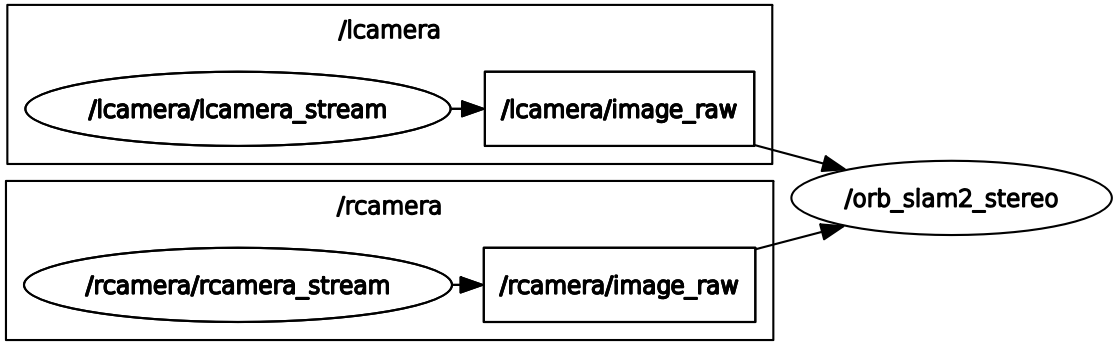
\includegraphics[width=0.8\textwidth]{./media/images/nodegraphstereoorbslam.png}
  	\caption{Node Graph with Stereo ORB-SLAM2}
  	\label{img:nodegraphstereoslam}
\end{figure}
Note that the \gls{slam} will freak out when the cameras are not \enquote{looking} at the same picture or are at different angles.


% ---------------------------------------------------
% Running LSD-SLAM
\section{Running LSD-SLAM\authorA}
Running the LSD-SLAM is not as straight forward as it is on the ORB-SLAM \ref{ref:runningmonocularorbslam}. The implementation of the LSD-SLAM is made to use it with \gls{ros} out of the box but the \href{https://github.com/tum-vision/lsd_slam}{original version} \cite{githublsdslamtum} by the Computer Vision Group at the Technical University of Munich was not updated in the past 5 years and such had some problems when running it on a newer version of \gls{ros} and Ubuntu. Therefor an more up-to-date version by Kevin George was used where he added support for newer versions of libraries and fixed some bugs. Even though the \href{https://github.com/kevin-george/lsd_slam}{fork by Kevin George} \cite{kevingeorgelsdslam} was updated 2 Years ago there were still some bugs and other problems. So a fork was created with the fixes to address the problems that where in Kevin George's Repository. The fork includes bug fixes to run LSD-SLAM on \gls{ros}-Melodic and Ubuntu 18.04 pretty much out of the box.\newline
The \href{https://github.com/MrMinemeet/lsd_slam}{new fork} \cite{alexandervoglspergerlsdslam} contains implementation to use \textsc{Eigen v3.2.5} that doesn't need to be installed, a special version of General Graph Optimization (\gls{g2o}) and a \textsc{CSPARSE}-directory path fix.\newline

% Listing of errors when building LSD-SLAM from original source
\subsection{Errors when building from source original source}
This list shows typical errors when building the LSD-SLAM from source and how to fix or at least bypass them.

%Cannot bind non_const lvalue to rvalu
\subsubsection{Cannot bind non\_const lvalue to rvalue}
When receiving an error like shown in listing \ref{error:non_const_lvalue_to_rvalue} this is most likely due to a datatype error where the functions expects a \textsc{double} but a \textsc{float} is defined.
to fix this, it is only necessary to change \textit{float x,y,z;} to \textit{double x,y,z;} in the two files in the error.\newline
\begin{lstlisting}[language=bash,label={error:non_const_lvalue_to_rvalue}]
PointCloudViewer.h:136:26: error: cannot bind non-const lvalue reference of type 'qreal& {aka double&}' to an rvalue of type 'qreal {aka double}'
   frame.getPosition(x,y,z);
   
PointCloudViewer.cpp:327:44: error: cannot bind non-const lvalue reference of type 'qreal& {aka double&}' to an rvalue of type 'qreal {aka double}'
        camera()->frame()->getPosition(x,y,z);
\end{lstlisting}

% no such function found: g2o::OptimizationAlgorithmLevenberg
% base_vertex.h not found
\subsubsection{\textit{no such function found: g2o::OptimizationAlgorithmLevenberg} and \textit{base\_vertex.h not found}}
This error occurs due to a change in newer \gls{g2o} versions. To fix this, it is required to install the \textit{g2o c++03} version. The fix  itself for this error can be found at \gls{g2o} \ref{ref:g2o}.

% cannot find -lcparse
\subsubsection{/usr/bin/ld: cannot find -lcsparse}
The error shown in \ref{error:cannotfindlcsparse} most likely accuress when catkin is looking for files that are in a different folder that expected by it.
\begin{lstlisting}[language=bash,label={error:cannotfindlcsparse}]
[ 91%] Linking CXX shared library /home/alex/lsd-slam_ws/devel/lib/liblsdslam.so
/usr/bin/ld: cannot find -lcsparse
collect2: error: ld returned 1 exit status
\end{lstlisting}
To fix it the paths where the required files are, have to be included in the \textit{CMakeList.txt} file which can be found in the source folder. Add the block shown in \ref{code:csparseincludedir} at the top of the file and replace \textsc{csparse} and \textsc{cxsparse} with \textsc{\$\{CSPARSE\_INCLUDE\_DIR\}} at the line where \textit{target\_link\_libraries} is adding the links to libraries.

\begin{lstlisting}[label={error:csparseincludedir}]
find_path(CSPARSE_INCLUDE_DIR NAMES cs.h
  PATHS
  /usr/include/suitesparse
  /usr/include
  /opt/local/include
  /usr/local/include
  /sw/include
  /usr/include/ufsparse
  /opt/local/include/ufsparse
  /usr/local/include/ufsparse
  /sw/include/ufsparse
  PATH_SUFFIXES
  suitesparse
  )
\end{lstlisting}

% liblsdslam.so: Warning: undefined reference »..«
\subsubsection{liblsdslam.so: Warning: undefined reference »..«}
This error is a batch of errors that occur at the same time.
It is mainly that references cannot be found by the system. The error might look something like shown below and is very easy to fix. The problem is that the \textit{libsuitesparse-dev} package is missing. When installing the package and then compiling \gls{g2o} it should work again.
\begin{lstlisting}[language=bash]
.../liblsdslam.so: Warning: undefined reference cs_di_post
.../liblsdslam.so: Warning: undefined reference cs_di_etree
.../liblsdslam.so: Warning: undefined reference cs_di_sfree
\end{lstlisting}

% double free or corruption
\subsubsection{double free or corruption}
\begin{lstlisting}[language=bash]
double free or corruption (out)
Aborted (core dumped)
\end{lstlisting}
The error shown in listing is due to changes in newer versions of Eigen. To fix this the easiest way is to download the version \textsc{3.2.5} from the \href{https://bitbucket.org/eigen/eigen/downloads/?tab=tags}{Eigen Bitbucket website} \cite{eigenbitbucket} and un-compress it somewhere where it can stay during the build process.
In the \textit{CMakeList.txt} of the \textit{lsd\_slam\_core} add the code like shown in listing \ref{code:lsdcorecmakelist} and replace \textsc{PATH} with the just unpacked folder path.
\begin{lstlisting}[language=bash, label={code:lsdcorecmakelist}, caption={CMakeList in lsd\_slam\_core with fix for Eigen}]
set(EIGEN3_INCLUDE_DIR "PATH")
include_directories(
  include
  ${EIGEN3_INCLUDE_DIR}
\end{lstlisting}

% g2oTypeSim3Sophus.h Errors
\subsubsection{g2oTypeSim3Sophus.h Errors}
Another error that likes to come up multiple times in the same file. 


% Installing LSD-SLAM with fixed repository
\subsection{Installing LSD-SLAM from fixed repository}
To run the LSD-SLAM a few packages are required. They can be installed using\newline
\begin{lstlisting}[language=bash, caption={Installing prerequisites for LSD-SLAM}]
    apt install ros-melodic-cv-bridge liblapack-dev libblas-dev freeglut3-dev libqglviewer-dev-qt4 libsuitesparse-dev libx11-dev
\end{lstlisting}

and then creating a link for \textit{libQGLViewer} to the file the LSD-SLAM is looking for. To create the softlink this command is used wich basically creates a link just without the \textsc{-qt4} at the end.\newline
\begin{lstlisting}[language=bash,caption={Creating softlink for libQGLViewer.so}]
    sudo ln -s /usr/lib/x86\_64-linux-gnu/libQGLViewer-qt4.so /usr/lib/x86\_64-linux-gnu/libQGLViewer.so
\end{lstlisting}

\subsubsection{G2O}\label{ref:g2o}
As the LSD-SLAM requires a special version of the \gls{g2o} framework all other versions that have been installed on \gls{ros} need to be removed completely. For this first the \textit{ros-melodic-g2o} package needs to be purged and the leftovers need to be deleted to not conflict with the special version that is going to be installed later using.\newline
\begin{lstlisting}[language=bash, caption={Removing leftover from \gls{g2o}}]
    rm -r /usr/local/lib/libg2o* /usr/local/include/g2o /usr/local/lib/g2o /usr/local/bin/g2o*
\end{lstlisting}

To install the correct version of \gls{g2o} it needs to be cloned from \url{https://github.com/felixendres/g2o.git} which creates a g2o folder in which a \textit{build}-folder has to be created. In the \textit{build} folder two commands have to be executed in order to install the framework.\newline
\begin{lstlisting}[language=bash]
    cmake ..
    sudo make install
\end{lstlisting}

\subsubsection{Eigen}\label{ref:eigen}
When done it is also necessary to download a specific version of the \textsc{Eigen}-library which has to be in a location where it is not likely to be moved as the full path is required. The Path should look a bit like this \textit{/home/alex/Projects/LSD-SLAM/eigen-eigen-bdd17ee3b1b3/}. This path needs to be set in the \textit{CMakeList.txt} in the \textit{lsd\_slam\_core} folder which was contained in the LSD-SLAM repository. In the file at line \textbf{106} there should be a placeholder like shown in \ref{code:eigenpathdir}, which has to be replaced with the path of \textsc{Eigen}.\newline
\lstinputlisting[language=XML, firstline=106, lastline=106, caption={CMakeList Eigen Directory}, label={code:eigenpathdir}]{./media/code_snippets/LSD-SLAM-Core-CMakeList.txt}

\subsubsection{Building LSD-SLAM}\label{ref:buildinglsdslam}
When these steps are done there is only one last command to be executed in the root directory of the workspace. To compile the LSD-SLAM in the \textit{src} folder the command is \newline
\begin{lstlisting}[language=bash]
    catkin_make
\end{lstlisting}
which may take some time. 


% ---------------------------------------------------
% DeepTAM
\section{DeepTAM\authorB}
In the following section the process of getting DeepTAM to run will be explained. Also the Problems of our workflow will be listed.

\subsection{Ubuntu 16.04}

The first attempt was to work with Ubuntu 16.04 and Python3, following the instructions given by Uni-Freiburg. At first a virtual environment manager needed to be installed with pip3(a package manager for Python3). Here pew is used and installed. Afterwards a new environment is created and entered. These are the commands:  

\begin{lstlisting}[language=bash]
    pip3 install pew
    pew new deeptam
    pew in deeptam
\end{lstlisting}

The next step was to install tensorflow(\gls{tf}), minieigen and scikit-image, also with pip3. Here the first error occurred. The error is that during the installation of minieigen Eigen/Core cannot be found. This problem can be worked around with the following commands.

\begin{lstlisting}[language=bash]
    sudo apt-get install libeigen3-dev
    sudo apt-get install python3-minieigen 
    sudo apt-get install libboost-all-dev
\end{lstlisting}

After these commands minieigen can be installed with pip3. The next step is to clone and build lmbspecialops. lmbspecialops is a collection of tensorflow ops. The ops focus on networks for predicting depth and camera motion but can also be useful for other tasks. 
 	% Nur zur Info



%	--------------------------------------------------------
% 	INFO: Gliederung und Allgemeines
%	-------------------------------------------------------	
%% !TEX root = ../Vorlage_DA.tex

%	########################################################
% 			INFO: Zitieren, Abbildungen, Listing
%	########################################################


%	--------------------------------------------------------
% 	Überschrift, Inhaltsverzeichnis
%	--------------------------------------------------------
\chapter{INFO: Gliederung und Inhalt\authorB}

%	--------------------------------------------------------
\section{Gliederung}
%	--------------------------------------------------------

Die vorhergehenden Kapitel sind Muss-Bestandteile der Diplomarbeit.
Ab hier kann die Gliederung (Aufteilung in Kapitel) frei gewählt werden.

Das Dokument soll durch Kapitel und Unterkapitel übersichtlich gegliedert sein. 
Jedes Kapitel bekommt eine Überschrift mit Nummerierung (1.1, 2.2.1, ...). Mehr als 3 Überschriftebenen (1.1.1) sollten vermieden werden. Zusätzlich muss bei jedem Hauptkapitel oder Kapitel mit einer Fußnote vermerkt werden, wer diesen Abschnitt erstellt hat.

Umfangreichere Arbeitsergebnisse wie Schaltpläne, Messprotokolle, Datenblätter und das Projekttagebuch kommen in einen Anhang am Ende des Dokuments.

In einem Literaturverzeichnis sind alle verwendeten Quellen und Zitate zu sammeln.

Wird die Diplomarbeit von \textbf{mehreren Personen} gemeinsam erstellt muss erkenntlich gemacht werden wer für welches Kapitel verantwortlich war.

%	--------------------------------------------------------
\section{Beispiel Gliederung}
%	--------------------------------------------------------

Hilfestellung für eine mögliche Benennung und Gliederung der Hauptkapitel:

\begin{description}
\item[Problemanalyse und Spezifikation]
\ \\Erläuterung des \underline{Was}: Aufgabenstellung ganz detailliert (=Pflichtenheft). Hier wird erläutert, was zu machen war. Das Wie ist hier normalerweise fehl am Platz.
\item[Entwurf]
\ \\Erläuterung des Wie: Technologie mit Begründung, bzw. Abwägen der Vor- und Nachteile. Lösungswege, Algorithmen.
\item[Implementierung]
\ \\Zeigt genau die Umsetzung des Entwurfs anhand wesentlicher Quelltext-Ausschnitte.
\item[Test und Inbetriebnahme]
\ \\Erkläre wie getestet wurde und was notwendig ist um das Produkt von Null weg zu installieren.
\item[Bedienungsanleitung]
\ \\Erklärt dem Benutzer die wichtigsten Schritte bei der Bedienung des Systems.
Eventuell ist eine eigenes Bedienerhandbuch für spezielle Benutzergruppen (z.B. Administratoren) notwendig.
\item[Fazit, Schlussfolgerungen]
\ \\Hier werden die Projektergebnisse zusammengefasst. Was ist gelungen was nicht. Welche Erkenntnisse wurden gewonnen.
\item[Persönliche Erfahrungen]
\ \\Hier (und nur hier) darf subjektiv aus der Ich Perspektive über das Projekt philosophiert werden.
\end{description}


%	--------------------------------------------------------
\section{Inhalt}
%	--------------------------------------------------------

Das Ziel ist die eigene Arbeit anderen (technisch versierten, aber projektfremden) Personen nachvollziehbar zu machen.
Ein Mitschüler der ein gutes Informatik Fachwissen hat soll den Text verstehen können.

Die Dokumentation eines Informatik-Projekts soll \textbf{Programmquelltext} enthalten!
Dieser soll gut dokumentiert und lesbar sein. 
Nur wenig zusätzlicher Text soll notwendig sein um das Programm zu verstehen.
Wählt nur jene Programmteile aus, die wirklich interessant sind, nehmt nicht jene Dinge die man in jedem Buch nachlesen kann.

Werden zur Implementierung Libraries, Frameworks, Methoden, etc. verwendet die wesentlich über den normalen Unterrichtsstoff hinausgehen, so sollten diese kurz erklärt werden.
Es ist aber nicht notwendig und nicht zielführend ganze Tutorials zu erstellen.
Nach einer allgemeinen Übersicht, die zu einem grundsatzlichen Verständnis verhelfen soll, genügt es auf entsprechende Quellen zu verweisen.

Der \textbf{Umfang} der Arbeit ist nicht wesentlich, wichtig ist die Qualität des Inhalts.
Ca.\ 40 Seiten pro Person sind eine gute Richtlinie.

Der Inhalt soll aus der \textbf{eigenen Feder} stammen. 
Kopieren fremder Quellen (auch wenn diese ins Deutsche übersetzt werden müssen) ist auf ein Minimum zu beschränken. 
Wenn kopiert wird dann ist immer genau anzugeben von wo. 
Siehe auch Kapitel \ref{ref:zitieren}.

Von Dir verfasste Texte sind Deine Visitenkarte. 
Bemühe Dich alles so gut zu machen wie Du nur kannst.
\begin{itemize}
\item
Strebe nach \textbf{Perfektion} --- auch was die Rechtschreibung und Grammatik angeht.
\item
Gib keinen Text aus der Hand mit dem Du nicht 100\% zufrieden bist.
\item
Lösche unfertige Textstellen ehe Du den Text weitergibst.
\item
Suche Dir jemanden zum Korrekturlesen, in eigenen Texten übersieht man gerne Fehler die einem Anderen sofort auffallen.
\end{itemize}

Keine Erklärungen aus der \textbf{Ich-Perspektive} abgeben (Ausnahme: Fazit am Ende).

Vermeide den Text so zu schreiben wie man spricht, bei Text gelten etwas andere Regeln als bei einer Präsentation.
Verzichte auf das übernehmen mundartlicher Ausdrucksweisen.

Überlege Dir beim Schreiben einer Textstelle ob der Leser das notwendige Hintergrundwissen hat um zu verstehen was Du ausdrücken willst.
Hast Du schon vorher erklärt was man an dieser Stelle wissen sollte?
Versteht man von was die Rede ist?
Beachte, dass Du top in das Thema eingearbeitet bist. 
Was Dir völlig klar erscheint ist dem Leser vielleicht nur ein spanisches Dorf.

Sei aber auch nicht zu weitschweifig. 
Ein guter Text ist kein langer Text sondern ein Text an dem man beim besten Gewissen nichts mehr wegkürzen kann.
Schreibe zuerst etwas weitschweifiger und kürze dann radikal.
Sei nicht zimperlich, wenn Dir eine Stelle nicht gefällt, lösche diese und fange von vorne an.

 	% Nur zur Info

%	--------------------------------------------------------
% 	INFO: Zitieren, Abbildungen, Listing
%	-------------------------------------------------------	
%% !TEX root = ../Vorlage_DA.tex

%	########################################################
% 			INFO: Zitieren, Abbildungen, Listing
%	########################################################


%	--------------------------------------------------------
% 	Überschrift, Inhaltsverzeichnis
%	--------------------------------------------------------
\chapter{INFO: Zitieren, Abbildungen, Quelltext\authorA}\label{ref:zitieren}

In diesem Kapitel sind Beispiele angeführt, wie Abbildungen, Zitate und Quelltext zu verwenden sind.

Die Zitate, Abbildungen und Listings werden automatisch in das Quellen- und Abbildungsverzeichnis übernommen. 
Das Literatur-, Abbildungs- und Listingsverzeichnis sind am Ende der Arbeit zu finden.   

%	--------------------------------------------------------
% 	Inhalt 
%	--------------------------------------------------------
\section{Abbildungen}\label{ref:abbildungen}

Abbildung sind mit einer Abbildungsnummer und einer Unterschrift zu versehen die kurz die Abbildung beschreibt. 
Abbildungen gehören zum umgebenden Text und müssen dort erwähnt werden.

Beispiel: In Abbildung \ref{htl01} wird das Logo der HTL Braunau dargestellt.

Wird auf eine Abbildung referenziert die sich weiter von der aktuellen Textstelle entfernt befindet so kann auch die Seitennummer hinzugefügt werden.

Beispiel: Siehe Abbildung \ref{htl01} auf Seite \pageref{htl01}.


%	--------------
%	Eine Abbildung
\begin{figure}[H]
	\centering
	
\includegraphics[width=0.5\textwidth]{./media/images/htl_c_cmyk_rein.pdf}
  	\caption{Logo der HTL Braunau.}
  	\label{htl01}
\end{figure}


%	----------------
%	Zwei Abbildungen

\begin{figure}[H]
  \centering
  \subfloat[Logo der HTL Braunau.]{\label{fig:a}
\includegraphics[width=.25\textwidth]{./media/images/htl_c_cmyk_rein.pdf}}
  \qquad
  \subfloat[Logo der HTL Braunau.]{\label{fig:b}
\includegraphics[width=.25\textwidth]{./media/images/htl_c_cmyk_rein.pdf}}
  \label{fig:canvas_01}
  % caption - In eckigen Klammern: Text für das Abbildungsverzeichnis
  \caption[Zwei Logos der HTL Braunau]{Zwei Logos der HTL Braunau in einer Abbildung zusammengefasst.}
\end{figure}


%	----------------
%	Drei Abbildungen
\begin{figure}[H]
  \centering
  \subfloat[Logo]{\label{fig:a}
\includegraphics[width=.15\textwidth]{./media/images/htl_c_cmyk_rein.pdf}}
  \qquad
  \subfloat[Logo]{\label{fig:b}
\includegraphics[width=.15\textwidth]{./media/images/htl_c_cmyk_rein.pdf}}
\qquad
  \subfloat[Logo]{\label{fig:b}
\includegraphics[width=.15\textwidth]{./media/images/htl_c_cmyk_rein.pdf}}
  \label{fig:canvas_04}
\caption[Drei Logos der HTL Braunau]{Dreimal das Logo der HTL Braunau.}
\end{figure}


\section{Zitate, Quellen, Fußnoten}

Es muss dem Leser möglich sein alle dargestellten Informationen selbst zu überprüfen.
Daher gilt der wissenschaftliche Grundsatz: 
Wer Informationen/Erkenntnisse verwendet die nicht von einem selbst stammen muss dies eindeutig kennzeichnen.
Das gilt für Bücher, Zeitschriftenartikel aber auch für alle Internetquellen.

Dem Leser Hinweise darüber zu geben wo genauere/weitere Informationen zu einem Thema zu finden sind ist ein weiterer Grund für Zitieren.

Es ist erlaubt fremde Quellen zu zitieren solange dies eindeutig erkennbar ist und sich die zitierten Stellen auf einen kurzen Absatz mit wenigen Zeilen beschränken. Auch wenn nicht wortwörtlich zitiert wird ist die Quelle der Information anzugeben.

Wörtliche Zitate werden durch Anführungszeichen begonnen und beendet sowie kursiv geschrieben: 
\emph{\glqq Wissenschaftliches Plagiat: Man kann sich zwar mit fremden Federn schmücken, aber man kann nicht mit ihnen fliegen.\grqq}~\cite{bib:uhlenbruck1}


Längere Zitate werden durch Einrücken vom normalen Text abgesetzt:
\begin{quotation}
\noindent
\emph{\glqq We tend to think of navigating a website as clicking from page-to-page via some kind of global navigation that’s always visible. When it comes to a single page, we often think scrolling is the one and only way to move from one end to the next.\grqq}~\cite{bib:bradley1}
\end{quotation}

Die eckigen Klammer mit Nummer kennzeichnet die Quelle.
Am Ende des Dokuments werden alle Quellen im Literaturverzeichnis aufgelistet. \cite{bib:wikilitverz}.

Das Verwenden fremden Gedankenguts ohne die Quelle anzugeben ist ein Plagiat (geistiger Diebstahl, \cite{bib:wikiplagiat}) und unter Umständen sogar eine Urheberrechtsverletzung.


Verweise in das Literaturverzeichnis sind nicht auf Zitate beschränkt sondern können auch eingesetzt werden um darauf hinzuweisen wo zu einem Thema mehr Informationen erhältlich sind.


Es ist zunehmend eine Kurzzitierweise in Fußnoten üblich: Nachname des Verfassers, Kurztitel, Seitenangabe.\footnote{John Doe, \glqq Verwendung von Fußnoten\grqq, Seite 12.}


%	%%%%%%%%%%%%%%%%%%%%%%%%%%%%%%%%%%%%%%%%%%%%%
%	Listings, Code
%	%%%%%%%%%%%%%%%%%%%%%%%%%%%%%%%%%%%%%%%%%%%%%
\section{Listings, Code}

Quelltext ist ein wesentlicher Bestandteil einer Informatik Diplomarbeit.
Listings werden wie Abbildungen nummeriert und mit einer Unterschrift versehen.
Ebenfalls müssen sie im Text referenziert werden.

\subsection{Beispiele}

Listing \ref{code:helloworld} auf Seite \pageref{code:helloworld} zeigt ein Hallo Welt Programm.

%	%%%%%%%%%%%%%%%%%%%%%%%%%%%%%%%%%%%%%%%%%%%%%
%	C++
\begin{minipage}{\linewidth}
\lstinputlisting[language=C++,caption={Mein erstes C-Programm.},label=code:helloworld]{./media/code_snippets/bsp_01.cpp}
\end{minipage}


Das PHP Programm \ref{code:phpread} dient zum ermitteln aller Dateien eines Unterverzeichnisses.

\begin{lstlisting}[language=PHP,caption={Alle Dateinamen ausgeben.},label=code:phpread]
<?php
if ($handle = opendir(realpath(__DIR__ . '/../userimages'))) {
    
    while (false !== ($file = readdir($handle))) {
        echo "$file//";
    }

    closedir($handle);
}
?>
\end{lstlisting}

\begin{lstlisting}[language=JavaScript,caption={Mausposition ermitteln.}]
// Calculates the mouse position.
function getMousePos(canvas, evt) {
	var rect = canvas.getBoundingClientRect();
	return {
		x: evt.clientX - rect.left,
		y: evt.clientY - rect.top
	};
}
\end{lstlisting}




%	%%%%%%%%%%%%%%%%%%%%%%%%%%%%%%%%%%%%%%%%%%%%%
%	CSS
\lstinputlisting[language=CSS,caption={Kurzer CSS--Quelltext.}]{./media/code_snippets/bsp.css}


%	%%%%%%%%%%%%%%%%%%%%%%%%%%%%%%%%%%%%%%%%%%%%%
%	HTML
\lstinputlisting[language=HTML,caption={HTML--Quelltext}]{./media/code_snippets/bsp.html}


%	%%%%%%%%%%%%%%%%%%%%%%%%%%%%%%%%%%%%%%%%%%%%%
%	HTML
\lstinputlisting[language=JavaScript,caption={JavaScript--Quelltext}]{./media/code_snippets/bsp.js}



 	% Nur zur Info


%	--------------------------------------------------------
% 	Fazit und Persönliche Erfahrungen
%	--------------------------------------------------------
% !TEX root = ../Vorlage_DA.tex

%	########################################################
% 					Fazit und Persönliche Erfahrungen
%	########################################################



%	--------------------------------------------------------
% 	Überschrift, Inhaltsverzeichnis
%	--------------------------------------------------------
\chapter{Fazit und Persönliche Erfahrungen}


%	--------------------------------------------------------
% 	Fazit
%	--------------------------------------------------------
\section{Fazit}

Zusammenfassung der Projektergebnisse. 
Besondere Erkenntnisse. Beurteilung des Lösungswegs. Eventuelle Alternativen und möglicher Erweiterungen.

%	--------------------------------------------------------
% 	Persönliche Erfahrungen
%	--------------------------------------------------------
\section{Persönliche Erfahrungen}

Hier (und nur hier) darf aus der Ich-Perspektive geschrieben werden.

%	--------------------------------------------------------
% 	Ausblick
%	--------------------------------------------------------
\section{Ausblick}

%	########################################################
% 	Anhang		
%	########################################################
\appendix

%	--------------------------------------------------------
% 	LaTeX
%	--------------------------------------------------------	
%% !TEX root = ../Vorlage_DA.tex

%	########################################################
% 					Diverse Anhänge
%	########################################################


%	--------------------------------------------------------
% 	Überschrift, Inhaltsverzeichnis
%	--------------------------------------------------------
\chapter{\LaTeX \authorA}

Das vorliegende Dokument wurde in \LaTeX\ erstellt.
\LaTeX\ (gesprochen Latech) ist ein Textsatzsystem das speziell für umfangreiche  und komplexe wissenschaftliche, technische und mathematische Dokumente entwickelt wurde.
Man schreibt Quelltext wie bei einem Programm und übersetzt diesen Quelltext in ein PDF Dokument.
Siehe \cite{bib:latexintro}.
 
%~~~~~~~~~~~~~~~~~~~~~~~~~~~~~~~~~~~~~~~~~~~~~~~~~~~~~~~~~~~~~~~~~~~~~~~~~~~~~~~~
\section{Die Vorlage}

Die \LaTeX\ Quelltexte dieses Dokuments sind gedacht um als Vorlage für die eigenen Diplomarbeit verwendet zu werden.
Dazu muss der Inhalt durch die eigene Arbeit ersetzt werden.
\verb+Vorlage_DA.tex+ ist das zentrale Haupt-Dokument, in dieses werden die einzelnen Kapitel inkludiert. Die Dateien für die eingefügten Kapitel finden sich im Unterordner \verb+chapters+.

Die Vorlage kann von GitHub geladen werden:
\url{https://github.com/matejkaf/latex-da-vorlage}

%~~~~~~~~~~~~~~~~~~~~~~~~~~~~~~~~~~~~~~~~~~~~~~~~~~~~~~~~~~~~~~~~~~~~~~~~~~~~~~~~
\section{Programme}

Programme (Editor + PDF Compiler) für \LaTeX:

Für Mac: MacTeX
\url{https://tug.org/mactex/}

Für Windows: MiKTeX
\url{http://miktex.org}\\
Zusätzlich auch die neueste Adobe Reader Version installieren!

Online:
Mit dem Service "`Overleaf"' (\url{https://www.overleaf.com/}) gab es positive Erfahrungen. Damit können die Dokument online erstellt und gemeinsam verwendet werden.



%~~~~~~~~~~~~~~~~~~~~~~~~~~~~~~~~~~~~~~~~~~~~~~~~~~~~~~~~~~~~~~~~~~~~~~~~~~~~~~~~
\section{Bitmap Fonts}


Bei MiKTeX unter Windows kann es ein Font Problem geben.
Falls die Schrift nicht scharf ist --- PDF so vergrößern dass ein Buchstabe gut 10 cm groß ist --- dann sieht man die Pixel, siehe Abbildung \ref{fig:bitmapfont}.
In diesem Fall wird ein sogenannter Bitmap-Font verwendet. 
Besser ist ein Vektor-Font, dieser lässt sich beliebig ohne Qualitätsverlust vergrößern.

\textbf{Lösung:}
Mit "`MiKTex Package Manager"' das Package \verb+cm-super+ installieren.

\begin{figure}[H]
	\centering
	
\includegraphics[width=0.75\textwidth]{./media/images/bitmap_font}
  	\caption{Oben Bitmap-, unten Vektor-Font}
  	\label{fig:bitmapfont}
\end{figure}

%~~~~~~~~~~~~~~~~~~~~~~~~~~~~~~~~~~~~~~~~~~~~~~~~~~~~~~~~~~~~~~~~~~~~~~~~~~~~~~~~
\section{LaTeX Quelltext}

Bei LaTeX wird der Text, dessen Gliederung in die Formatierung in puren Textfiles mit der Endung \verb+.tex+ beschrieben.
Die Zeichenkodierung der Files muss UTF-8 sein.

Der "`LaTeX Compiler"' (Programm mit dem Namen pdflatex) übersetzt diese Files in ein PDF Dokument.

%~~~~~~~~~~~~~~~~~~~~~~~~~~~~~~~~~~~~~~~~~~~~~~~~~~~~~~~~~~~~~~~~~~~~~~~~~~~~~~~~
\section{Gerüst}

Die Grundstruktur eines \LaTeX\ Dokuments:
\begin{Verbatim}[frame=single]
\documentclass[a4paper,10pt,final,oneside]{scrartcl}	

\usepackage{anysize}
\usepackage[utf8]{inputenc}
\usepackage[T1]{fontenc}
\usepackage[ngerman]{babel}
\usepackage[pdftex]{hyperref}
\usepackage{url}
 
\begin{document}

Ab hier kommt der Inhalt

\end{document}
\end{Verbatim}

Hinweis:
Durch die Vorlage ist diese Grund-Struktur bereits vorgegeben.

%~~~~~~~~~~~~~~~~~~~~~~~~~~~~~~~~~~~~~~~~~~~~~~~~~~~~~~~~~~~~~~~~~~~~~~~~~~~~~~~~
\section{Formatierungen}

\begin{minipage}[t]{0.6\linewidth}
\begin{Verbatim}[frame=single]
Mehrere     Leerzeichen werden 
ignoriert
ein einfacher Zeilenumbruch gilt 
als Leerzeichen.

Eine leere Zeile kennzeichnet einen 
neuen Absatz.
\end{Verbatim}
\end{minipage}
\begin{minipage}[t]{0.4\linewidth}
Mehrere     Leerzeichen werden ignoriert
ein einfacher Zeilenumbruch 
gilt als Leerzeichen.

Eine leere Zeile kennzeichnet 
einen neuen Absatz.
\end{minipage}

\vspace{1em}\noindent
Diverse Formatierungen:

\begin{tabular}{l|l}
\texttt{Typewriter} & \lstinline!\texttt{...}! o.\ \lstinline!{\ttfamily ...}!\\ 
\textbf{Fett} & \lstinline!\textbf{...}! o.\ \lstinline!{\bfseries ...}!\\ 
\textit{Italic} & \lstinline!\textit{...}! o.\ \lstinline!{\itshape ...}!\\ 
\textsl{Slanted} & \lstinline!\textsl{...}! o.\ \lstinline!{\slshape ...}!\\ 
\textsc{Kapitälchen} & \lstinline!\textsc{...}! o.\ \lstinline!{\scshape ...}!\\ 
\textmd{Normal} & \lstinline!\textmd{...}! o.\ \lstinline!{\mdseries ...}!\\ 
\emph{Emph} & \lstinline!\emph{...}! o.\ \lstinline!{\em ...}!\\ 
\textsf{Sans Serif} & \lstinline!\textsf{...}! o.\ \lstinline!{\sffamily ...}!\\
\underline{Unterstrichen} & \lstinline!\underline{...}!\\
Größen & \lstinline!\tiny! \lstinline!\scriptsize! \lstinline!\footnotesize! \lstinline!\small! \lstinline!\normalsize! \lstinline!\large! \lstinline!\Large!\\
 & \lstinline!\LARGE! \lstinline!\huge! \lstinline!\Huge!\\ 
Zentriert & \lstinline!\begin{center}...\end{center}!\\
Gesch.\ Leerz. & \lstinline!~!\\
Zeilenumbruch & \lstinline!\\! oder \lstinline!\newline!\\
Absatzumbruch & \lstinline!\par! oder leere Zeile.\\

\end{tabular}


%~~~~~~~~~~~~~~~~~~~~~~~~~~~~~~~~~~~~~~~~~~~~~~~~~~~~~~~~~~~~~~~~~~~~~~~~~~~~~~~~
\section{Überschriften}

\begin{Verbatim}[frame=single]
\chapter{Hauptkapitel}
\section{Kapitel}
\subsection{Unterkapitel}
\subsubsection{Unterunterkapitel}
\end{Verbatim}

Die Kapitelnummerierung und das Inhaltsverzeichnis werden automatisch erstellt.

%~~~~~~~~~~~~~~~~~~~~~~~~~~~~~~~~~~~~~~~~~~~~~~~~~~~~~~~~~~~~~~~~~~~~~~~~~~~~~~~~
\section{Autoren\authorB}

Für eine Diplomarbeit mit mehreren Autoren muss nachvollziehbar sein wer für welchen Teil der Urheber ist.
Dies ist durch \textbf{Namenskürzel} (2-stellig) in den Überschriften darzustellen (siehe in diesem Dokument).

Eine Person soll immer für ein komplettes Hauptkapitel (\verb+chapter+) oder Kapitel (\verb+section+) verantwortlich sein. 
Eine Aufteilung auf Ebene der Unterkapitel (\verb+subsection+) oder Unterunterkapitel (\verb+subsubsection+) sollte vermieden werden.

Die Namenskürzel werden in \verb+Vorlage_DA.tex+ definiert:

\begin{Verbatim}[frame=single]
% Initialen der Authoren
\def\authorInitialsA{MM} % Max Mustermann
\def\authorInitialsB{FF} % Frieda Fröhlich
\def\authorInitialsC{FE} % Fritz Einstein
\def\authorInitialsD{WA} % Weiterer Autor
\end{Verbatim}
 

Für das Einfügen der Namenskürzel ins Dokument dienen in weiterer Folge die Befehle 
\verb+\authorA+, 
\verb+\authorB+, 
\verb+\authorC+, 
\verb+\authorD+.

Beispiel --- erzeugt die Überschrift dieses Kapitels:
\begin{Verbatim}[frame=single]
\section{Autoren\authorB}
\end{Verbatim}

%~~~~~~~~~~~~~~~~~~~~~~~~~~~~~~~~~~~~~~~~~~~~~~~~~~~~~~~~~~~~~~~~~~~~~~~~~~~~~~~~
\section{Bilder einfügen}

Formate: pdf, jpg und png.
Dateien im Verzeichnis \verb+media/images+ ablegen.

\begin{Verbatim}[frame=single]
In Abbildung \ref{fig:htl01} sieht man das Logo der HTL Braunau.
\begin{figure}[H]
  \centering
  
\includegraphics[width=0.3\textwidth]{./media/images/htl_c_cmyk_rein.pdf}
  \caption{Logo der HTL Braunau.}
  \label{fig:htl01}
\end{figure}
\end{Verbatim}

\begin{framed}
In Abbildung \ref{fig:htl01} sieht man das Logo der HTL Braunau.
\begin{figure}[H]
	\centering
	
\includegraphics[width=0.3\textwidth]{./media/images/htl_c_cmyk_rein.pdf}
  	\caption{Logo der HTL Braunau.}
  	\label{fig:htl01}
\end{figure}
\end{framed}

Hinweis: Dateipfade mit \verb+"/"+ bilden!

Siehe
\url{http://en.wikibooks.org/wiki/LaTeX/Importing_Graphics}

Der Befehl \lstinline{\label} gibt der Abbildung einen eindeutigen Namen.
Durch \lstinline{\ref} wird dieser Name referenziert, d.h. es wird die automatisch generierte Abbildungsnummer eingefügt (dazu muss das \LaTeX\ Dokument 2-mal erstellt werden!)

Siehe \ref{ref:abbildungen}, Seite \pageref{ref:abbildungen} für Abbildungen die mehrere Bilder enthalten.

%~~~~~~~~~~~~~~~~~~~~~~~~~~~~~~~~~~~~~~~~~~~~~~~~~~~~~~~~~~~~~~~~~~~~~~~~~~~~~~~~
\section{Querverweise}

Mit Hilfe von Querverweisen verweist man auf andere Stellen im Dokument. 
Z.B. in der Form: "`Siehe \ref{ref:abbildungen}"' --- es wird die Kapitelnummer bzw. Abbildungsnummer angegeben.

Es kann auf Abbildungen und auf Überschriften verwiesen werden.
Diese erhalten zuerst mit \lstinline{\label} einen Namen.
\begin{Verbatim}[frame=single]
\section{Kapitelname} \label{ref:meinebezeichnung}
\end{Verbatim}

Möchte man auf diese Elemente verweisen gibt man den Namen im \lstinline{\ref} Befehl an.
\begin{Verbatim}[frame=single]
Eine genaue Beschreibung dieses Themas ist 
in Kapitel \ref{ref:meinebezeichnung} zu finden.
\end{Verbatim}

Ein Doppelpunkt als Teil des Namens ist erlaubt. Auf diese Weise können zum Beispiel Namen von Abbildungen, Überschriften und Listings unterschieden werden (\mbox{\lstinline{fig:}/\lstinline{ref:}/\lstinline{code:}}).

\LaTeX\ macht aus Querverweisen automatisch PDF Links.


%~~~~~~~~~~~~~~~~~~~~~~~~~~~~~~~~~~~~~~~~~~~~~~~~~~~~~~~~~~~~~~~~~~~~~~~~~~~~~~~~
\section{Aufzählungen}

\begin{minipage}[c]{0.3\linewidth}
\begin{Verbatim}[frame=single]
\begin{itemize}
\item Eins
\item Zwei
\item Drei
\end{itemize}
\end{Verbatim}
\end{minipage}
\begin{minipage}[c]{0.5\linewidth}
\begin{itemize}
\item Eins
\item Zwei
\item Drei
\end{itemize}
\end{minipage}

\noindent
\begin{minipage}[c]{0.3\linewidth}
\begin{Verbatim}[frame=single]
\begin{enumerate}
\item Eins
\item Zwei
\item Drei
\end{enumerate}
\end{Verbatim}
\end{minipage}
\begin{minipage}[c]{0.5\linewidth}
\begin{enumerate}
\item Eins
\item Zwei
\item Drei
\end{enumerate}
\end{minipage}

%~~~~~~~~~~~~~~~~~~~~~~~~~~~~~~~~~~~~~~~~~~~~~~~~~~~~~~~~~~~~~~~~~~~~~~~~~~~~~~~~
\section{Mathematische Formeln}

\begin{Verbatim}[frame=single]
Abgesetzte Formel:
\begin{equation*}
\frac{1+x}{1-x} \cdot \sqrt[3]{2} \cdot \binom{n}{k}
\end{equation*}
\end{Verbatim}

Abgesetzte Formel:
\begin{equation*}
\frac{1+x}{1-x} \cdot \sqrt[3]{2} \cdot \binom{n}{k}
\end{equation*}

\begin{Verbatim}[frame=single]
Formel im Textfluss:
$\frac{1+x}{1-x}, \sqrt[3]{2}, \binom{n}{k}$
\end{Verbatim}

Formel im Textfluß: $\frac{1+x}{1-x}, \sqrt[3]{2}, \binom{n}{k}$
\\

%~~~~~~~~~~~~~~~~~~~~~~~~~~~~~~~~~~~~~~~~~~~~~~~~~~~~~~~~~~~~~~~~~~~~~~~~~~~~~~~~
\section{Programm Quelltext}

Die Umgebung lstlisting übernimmt das Formatieren von Programmquelltext.

\begin{minipage}[t]{\linewidth}
\begin{Verbatim}[frame=single]
Listing \ref{code:complex} zeigt die Implementierung eines 
besonders komplexen Algorithmus.
\begin{lstlisting}[
    language=java,
    caption={Komplizierter Quelltext.},
    label=code:complex
]
while(x>0) {
	x--;
	// bla bla
}
\end{lstlisting}
\end{Verbatim}
\end{minipage}

\begin{framed}
Listing \ref{code:complex} zeigt die Implementierung eines 
besonders komplexen Algorithmus.
\begin{lstlisting}[
    language=java,
    caption={Komplizierter Quelltext.},
    label=code:complex
]
while(x>0) {
	x--;
	// bla bla
}
\end{lstlisting}
\end{framed}

Siehe auch \url{https://en.wikibooks.org/wiki/LaTeX/Source_Code_Listings}

%~~~~~~~~~~~~~~~~~~~~~~~~~~~~~~~~~~~~~~~~~~~~~~~~~~~~~~~~~~~~~~~~~~~~~~~~~~~~~~~~
\section{Code im Text}

\begin{minipage}[t]{\linewidth}
\begin{Verbatim}[frame=single]
Mit dem Befehl lstinline können kurze Programmfragmente 
direkt in den Textfluss integriert werden.
Das sieht dann so aus: 
\lstinline[language=java]{labels.add("" + i)}.
Allzu lange sollten diese Programmausschnitte aber nicht sein.
\end{Verbatim}
\end{minipage}

Mit dem Befehl lstinline können kurze Programmfragmente 
direkt in den Textfluß integriert werden.
Das sieht dann so aus: 
\lstinline{labels.add("" + i)}.
Allzu lange sollten diese Programmausschnitte aber nicht sein.


%~~~~~~~~~~~~~~~~~~~~~~~~~~~~~~~~~~~~~~~~~~~~~~~~~~~~~~~~~~~~~~~~~~~~~~~~~~~~~~~~
\section{Seitenümbruche}

Ein Seitenumbruch kann mit \lstinline{\pagebreak} erzwungen werden.

Soll etwas als ganzes auf der Seite stehen und nicht umgebrochen werden, so kann dieser Teil in eine \lstinline{minipage} Umgebung eingeschlossen werden.

\begin{Verbatim}[frame=single]
\begin{minipage}{\linewidth}
In diesem Teil findet kein Seitenumbruch statt.
\end{minipage}
\end{Verbatim}

Häufig wird dies bei Programmlistings nötig sein:

\begin{Verbatim}[frame=single]
Das Listing \ref{code:codenopagebreak} ist in eine minipage 
eingebunden. Dies wirkt sich so aus, dass dieses Listing nur 
als ganzes auf der Seite steht, sollte es nicht mehr Platz 
haben wird es komplett auf die folgende Seite gesetzt und 
es entsteht ein Leerraum auf der vorhergehenden Seite.

\begin{minipage}{\linewidth}
\begin{lstlisting}[
	language=java,
	caption={Java Quelltext.},
	label=code:codeexample1
]
public void prepend(Node n) {
	n.next=start;
	start=n;
}
\end{lstlisting}
\end{minipage}
\end{Verbatim}

Das Listing \ref{code:codenopagebreak} ist in eine minipage eingebunden.
Dies wirkt sich so aus, dass dieses Listing nur als ganzes auf der Seite steht, sollte es nicht mehr Platz haben wird es komplett auf die folgende Seite gesetzt und es entsteht ein Leerraum auf der vorhergehenden Seite.

\begin{minipage}{\linewidth}
\begin{lstlisting}[
	language=java,
	caption={Java Quelltext.},
	label=code:codenopagebreak
]
public void prepend(Node n) {
	n.next=start;
	start=n;
}
\end{lstlisting}
\end{minipage}


%~~~~~~~~~~~~~~~~~~~~~~~~~~~~~~~~~~~~~~~~~~~~~~~~~~~~~~~~~~~~~~~~~~~~~~~~~~~~~~~~
\section{Quellen und Literatur}

Alle Quellen befinden sich im Dokument \verb+chapters/Post-01-literatur.tex+ .
Eine Quelle erhält mit \lstinline|\bibitem{bib:name}| einen Namen.

Im Text wird durch den Befehl \lstinline{\cite} zitiert.
Bsp.:

\begin{Verbatim}[frame=single]
Siehe \cite{bib:latexintro}.
\end{Verbatim}

\begin{framed}
Siehe \cite{bib:latexintro}.
\end{framed}



%~~~~~~~~~~~~~~~~~~~~~~~~~~~~~~~~~~~~~~~~~~~~~~~~~~~~~~~~~~~~~~~~~~~~~~~~~~~~~~~~
\section{Links}

Links können in der Form einer URL eingefügt werden.
Dies kann (in kleinerem Umfang) statt Einträgen im Literaturverzeichnis verwendet werden.

\begin{Verbatim}[frame=single]
\url{http://www.orf.at}
\end{Verbatim}
\begin{framed}
\url{http://www.orf.at}
\end{framed}

Lange URL's sehen nicht besonders gut aus. Etwa \url{https://www.youtube.com/watch?v=_vQaOvPsLko&list=PL6gx4Cwl9DGBsvRxJJOzG4r4k_zLKrnxl&index=49}.

In diesem Fall bietet es sich an solche URL's mit einem Kurz-URL-Dienst (z.B. \url{tinyurl.com}) zu verkürzen. 
Obige URL in verkürzter Form: \url{http://tinyurl.com/hqtzqan}


%~~~~~~~~~~~~~~~~~~~~~~~~~~~~~~~~~~~~~~~~~~~~~~~~~~~~~~~~~~~~~~~~~~~~~~~~~~~~~~~~
\section{Fußnoten}

\begin{Verbatim}[frame=single]
Eine Fußnote kann man einfach%
\footnote{Hier zum Beispiel}
irgendwo in den Text einfuegen.
\end{Verbatim}

Eine Fußnote kann man einfach%
\footnote{Hier zum Beispiel}
irgendwo in den Text einfügen, diese wird an das untere Ende der Seite gesetzt.


%~~~~~~~~~~~~~~~~~~~~~~~~~~~~~~~~~~~~~~~~~~~~~~~~~~~~~~~~~~~~~~~~~~~~~~~~~~~~~~~~
\section{Tabellen}

Mit der Umgebung \lstinline{tabular} bzw. erweitert: \lstinline{tabularx}.

Siehe \url{https://en.wikibooks.org/wiki/LaTeX/Tables}

%: TODO Tabellen

%~~~~~~~~~~~~~~~~~~~~~~~~~~~~~~~~~~~~~~~~~~~~~~~~~~~~~~~~~~~~~~~~~~~~~~~~~~~~~~~~
\section{Mehrspaltiger Text}

\begin{multicols}{2}

Um einen zweispaltigen Text zu erzeugen kann die \verb+multicols+ Umgebung verwendet werden

\begin{Verbatim}[frame=single]
\begin{multicols}{2}
Text in 2 Spalten
\end{multicols}
\end{Verbatim}

Hier wurde multicols verwendet um die Abbildung platzsparend neben dem Text zu platzieren.
Siehe Logo der HTL Braunau in Abbildung \ref{logoTwoCols}.

%	--------------
%	Eine Abbildung

\columnbreak
\begin{figure}[H]
	\centering
	
\includegraphics[width=0.3\textwidth]{./media/images/htl_c_cmyk_rein.pdf}
  	\caption{Logo auf der rechten Seite.}
  	\label{logoTwoCols}
\end{figure}

Um einen Spaltenumbruch an einer bestimmten Stelle zu erzwingen:
\begin{Verbatim}[frame=single]
\columnbreak
\end{Verbatim}


\end{multicols}




%	--------------------------------------------------------
% 	Abschließende Prüfungen - Diplomarbeit
%	--------------------------------------------------------	
% Just takes up too much space
%% !TEX root = ../Vorlage_DA.tex

%	########################################################
% 					Richtlinien für Diplomarbeit
%	########################################################


%	--------------------------------------------------------
% 	Überschrift, Inhaltsverzeichnis
%	--------------------------------------------------------
\chapter{Abschließende Prüfungen - Diplomarbeit}

Anbei ein Auszug aus offizieller Information bezüglich der Diplomarbeit.

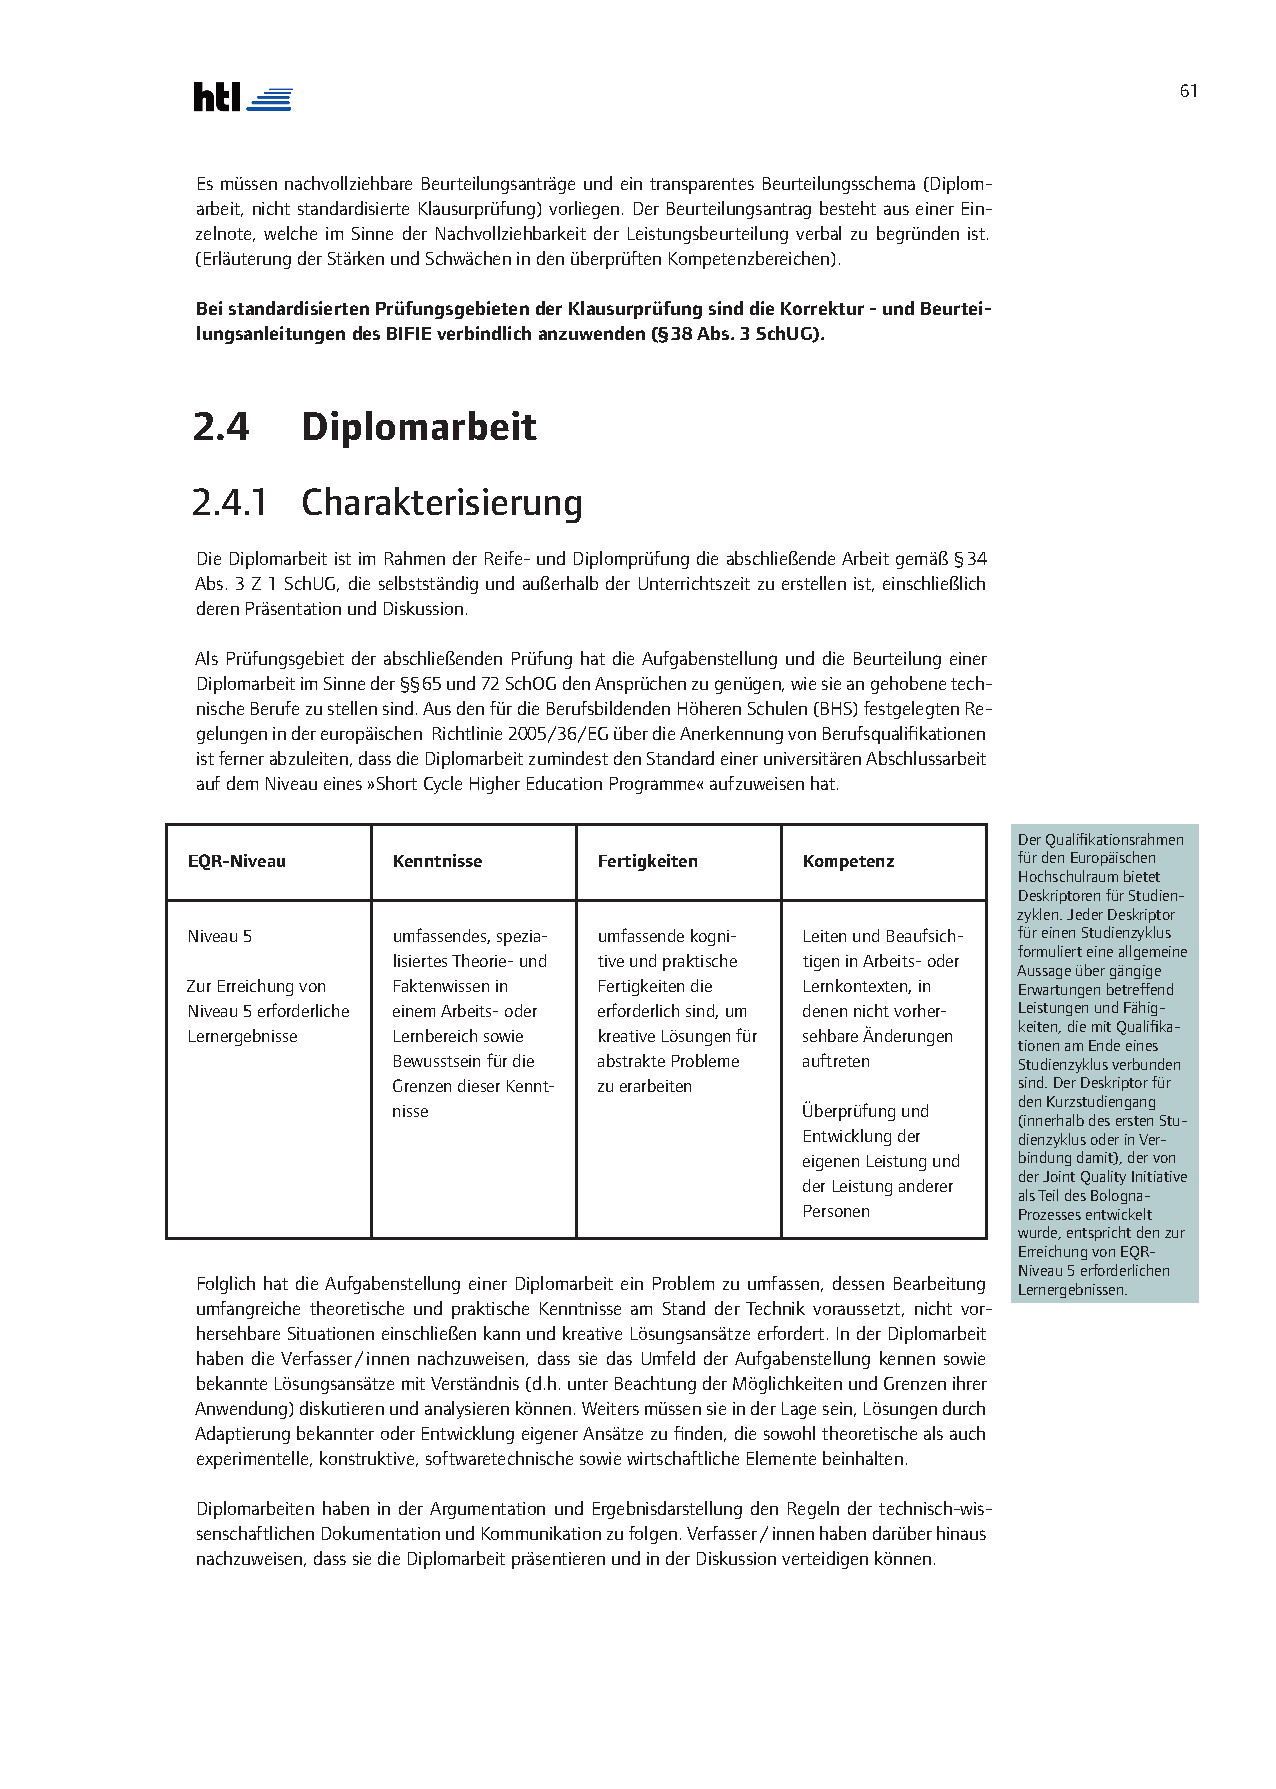
\includepdf[pages=-]{./media/info.pdf}




%	########################################################
% 	Erklärungen 		
%	########################################################
\printglossary


%	########################################################
% 	Quellenverzeichnis 		
%	########################################################
% \addcontentsline{toc}{chapter}{Literaturverzeichnis}
\bibliography{literature.bib} 
\bibliographystyle{ieeetr}


%	########################################################
% 	Abbildungsverzeichnis 		
%	########################################################
\addcontentsline{toc}{chapter}{Abbildungsverzeichnis}
\listoffigures

%	########################################################
% 	Verzeichnis der Listings 		
%	########################################################
\addcontentsline{toc}{chapter}{Quelltextverzeichnis}
\lstlistoflistings

%	--------------------------------------------------------
% 	Autoren
%	--------------------------------------------------------
% !TEX root = ../Vorlage_DA.tex
%	########################################################
% 					Autoren
%	########################################################


%	--------------------------------------------------------
% 	Überschrift, Inhaltsverzeichnis
%	--------------------------------------------------------
\chapter*{Authors} \markboth{Authors}{Authors}
\addcontentsline{toc}{chapter}{Authors}

%	--------------------------------------------------------
% 	Autor 1
%	--------------------------------------------------------
\htlParagraph{Alexander Voglsperger}

\renewcommand{\arraystretch}{1.2}
\begin{tabularx}{1\textwidth}{@{} l X l @{}}

\emph{Birthday, Place of birth:} & 25.03.2001, Ried im Innkreis & 
\multirow{5}{2.5cm}{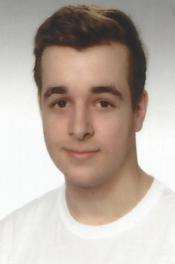
\includegraphics[width=2.5cm]{./media/images/alexander.png}
} 
\\
\emph{School education:} & Volksschule Aurolzmünster \newline Informatik Hauptschule Aurolzmünster \newline HTL Braunau & \\
\emph{Internship:} & Team7 Natürlich Wohnen GmbH, 4 Weeks, IT\newline
Krankenhaus Ried im Innkreis, 4 Weeks, IT\newline
Johannes Kepler University - AI Lab, 4 Weeks, Mapping and Tracking on self-driving car&\\
\emph{Address:} & Forchtenau 196\newline 4971, Aurolzmünster\newline Österreich & \\
\emph{E-Mail:} & alexander.voglsperger@gmail.com & \\

\end{tabularx}
\\\\

%	--------------------------------------------------------
% 	Autor 2
%	--------------------------------------------------------
\htlParagraph{Simon Moharitsch}

\begin{tabularx}{1\textwidth}{@{} l X l @{}}
\emph{Birthday, Place of birth:} & 01.01.1970, Braunau am Inn & 
\multirow{5}{2.5cm}{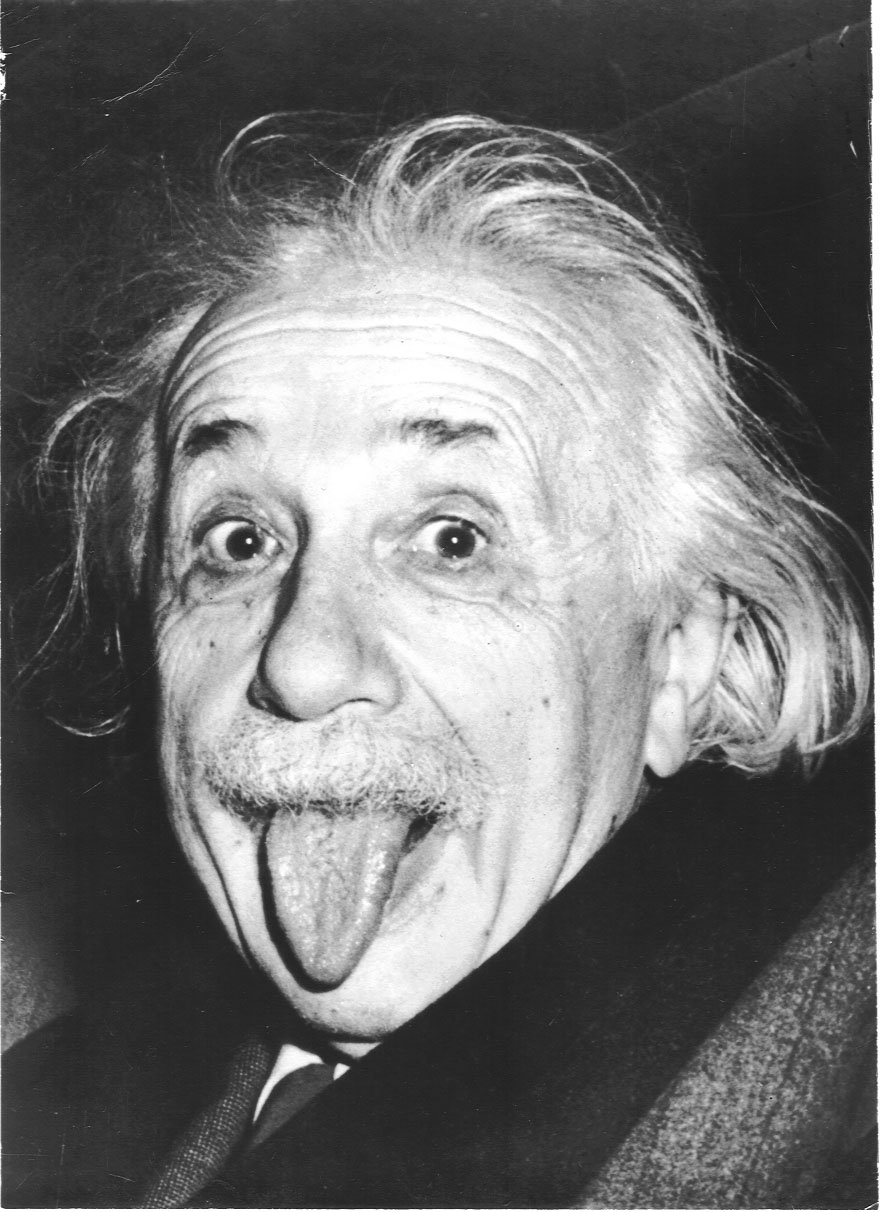
\includegraphics[width=2.5cm]{./media/images/einstein.jpg}
} 
\\
\emph{School education:} & Volksschule \newline Hauptschule \newline HTL & \\
\emph{Internship:} & Firmenname, Zeit, Tätigkeit & \\
\emph{Address:} & Strasse Nummer\newline PLZ, Ort\newline Österreich & \\
\emph{E-Mail:} & max@mustermann.com & \\

\end{tabularx}




\end{document}  